\documentclass[11pt]{article}

% Self-contained ICLR-style preamble — no external .sty file needed.
\usepackage[letterpaper,margin=1in]{geometry}
\usepackage{times}
\usepackage[T1]{fontenc}
\usepackage{microtype}
\usepackage{hyperref}
\hypersetup{colorlinks=true,linkcolor=black,urlcolor=blue!60!black,citecolor=blue!60!black}

\usepackage{booktabs}
\usepackage{tabularx}
\usepackage{amsmath}
\usepackage{amssymb}
\usepackage[table]{xcolor}
\usepackage{multirow}
\usepackage{colortbl}
\usepackage{enumitem}
\usepackage{float}
\usepackage{caption}
\usepackage{graphicx}
\graphicspath{{figures/}{./}}
\usepackage{natbib}
\bibliographystyle{plainnat}

% Drop heavy packages that may not be on every system; replace listings with verbatim
% and algorithm/algpseudocode with a simple verbatim block.

\definecolor{bestcolor}{RGB}{0,130,60}
\definecolor{warncolor}{RGB}{180,80,0}

\newcommand{\cmark}{\textcolor{bestcolor}{$\checkmark$}}
\newcommand{\xmark}{$\times$}
\newcommand{\nmark}{--}

\title{When Does Write-Time Augmentation Help Retrieval?\\
       A Divergence Diagnostic for RAG Pipelines}

\author{Jeffrey Chang}
\date{April 2026}

\begin{document}
\maketitle

%-----------------------------------------------------------------------------
\begin{abstract}
Write-time document augmentation --- adding LLM-generated questions
(docT5query), structured metadata, or multiple chunk representations
--- is a popular retrieval-pipeline lever, but published gains
($+3$--$10$ pp on single corpora) replicate inconsistently. We ask
\emph{when} augmentation helps and propose a free, pre-deployment
diagnostic: estimate the mean Jaccard divergence between $\sim 50$
held-out (query, target) pairs and act conditionally on the result.
We test the diagnostic and its conditional recommendations on five
corpora: a stratified enterprise benchmark of $160$ queries (with an
$80$-query held-out split), three BEIR test sets (SciFact, NFCorpus,
FiQA), LoTTE-writing-forum, and HotpotQA-500 multi-hop. Three findings
support the diagnostic. (i)~\textbf{Per-query rank improvement is a
detectable monotone function of query-target Jaccard divergence
within a corpus}: regression slopes are positive and significant on
the corpus where augmentation works (enterprise: $\beta{=}{+}1.41$,
$p{=}0.008$, $R^{2}{=}0.05$), and indistinguishable from zero on
corpora where it does not (SciFact: $\beta{=}{+}0.24$, $p{=}0.62$,
$R^{2}{<}0.01$). The same regression separates the
``augmentation-friendly'' from ``augmentation-neutral'' regime that
prior work has reported as cross-corpus heterogeneity.
(ii)~\textbf{RODS, a six-field schema we introduce, and docT5query
are statistically indistinguishable on R@5 in-distribution}
($p{=}0.52$), and \textbf{both R@5 lifts collapse on a held-out
split} ($p{=}0.73$). RODS-M4 retains a held-out MRR@10 lift
($+5.0$ pp, raw $p{=}0.011$), suggestive but borderline under
multiple-comparisons correction. (iii)~\textbf{Cross-encoder reranking
absorbs the single-chunk schema gain} ($p{=}0.67$) \textbf{but not
the multi-vector advantage} ($+6.5$ pp R@5 post-rerank, $p{<}0.001$;
$+8.1$ pp held-out MRR@10, $p{=}0.001$); a $4{\times}$ stronger
embedder (\texttt{all-mpnet-base-v2}) flips the comparison, widening
the single-chunk schema gap and erasing the quad-vector advantage.
\textbf{Under Holm--Bonferroni correction, only the multi-vector
MRR@10 lift survives at family-wise} $\alpha{=}0.05$; we therefore
present multi-vector as the robust positive result and the
single-chunk schema gains as suggestive. The diagnostic resolves
much of the cross-corpus heterogeneity reported in prior work:
format design, multi-vector indexing, reranking, and embedder scale
are complementary levers whose relative payoff is set by
query--document divergence and embedder budget. We release the diagnostic harness, the held-out
benchmark, and per-query rank traces.
\end{abstract}

%-----------------------------------------------------------------------------
\section{Introduction}
\label{sec:intro}
%-----------------------------------------------------------------------------

Consider an internal wiki where the section headed
\textit{``Decision: ADR-005''} contains the line
\textit{``We standardize on Python 3.12 for the backend''} and a
metadata block reading \texttt{Status: accepted}. A user types
\textit{``what is our standardized backend Python version?''}. None
of the query's content tokens appear in the heading, and only one
appears in the prose; under a default heading-aware RAG pipeline this
section ranks fifth, behind sections that share token \emph{Python}
but discuss something else. Write-time augmentation --- adding an
explicit \texttt{Summary}, \texttt{Type}, or \texttt{Entities} field
above the prose --- closes this gap. Whether it helps is the question
this paper studies.

More generally: a RAG pipeline is a sequence of fixed components ---
a chunker, an embedder, a retriever, optionally a reranker, and a
language model --- each with its own literature of optimisations.
\emph{Write-time document augmentation} (modifying what is written
into the index, rather than how it is retrieved) has produced
single-corpus gains of $+3$--$10$ pp R@5 across this literature
(docT5query, HyDE, ad-hoc per-section schemas, multi-vector
decompositions,
Contextual Retrieval), but the gains replicate inconsistently across
corpora and rarely survive a held-out split or a cross-encoder
reranker. The field has no predictive theory of \emph{when} write-time
augmentation is worth paying for.

\paragraph{Our proposal: a pre-deployment diagnostic.} On $\sim 50$
held-out (query, target) pairs, regress per-query rank improvement
(relative to a heading-aware baseline) on Jaccard divergence between
query and target tokens, and read off slope $\beta$ and significance.
A positive, significant $\beta$ predicts that write-time augmentation
will lift retrieval on this corpus; $\beta$ indistinguishable from
zero predicts that it will not. The diagnostic is parameter-free,
uses no LLM and no embedder, and runs in seconds.

\paragraph{RODS as a worked instance.} To give the diagnostic a
concrete object we release \emph{RODS} (Retrieval-Oriented Document
Structuring), a per-section schema of up to six typed fields with an
incremental ablation chain $M_0\to M_7$; the held-out check
(\S\ref{sec:heldout}) selects the deployable cut.

\paragraph{Branched recommendation.}
Beyond the go/no-go test, our cross-encoder rerank and embedder-swap
experiments yield a recommendation that branches on embedder budget
rather than picking a single ``best format'' (\S\ref{sec:conclusion}).

\paragraph{Contributions.} We make three contributions.
\begin{enumerate}[noitemsep,topsep=0.3em]
  \item \textbf{A pre-deployment divergence diagnostic for write-time
        augmentation, validated on five corpora.} We regress per-query
        rank improvement on Jaccard divergence
        $\mathrm{div}(q,d){=}1{-}|T(q){\cap} T(d)|/|T(q)|$ and report
        slope $\beta$, intercept $\alpha$, and $R^{2}$. The diagnostic
        is positive on corpora where augmentation works
        ($\beta_{\mathrm{RODS-M6}}{=}{+}1.41$, $p{=}0.008$ on enterprise)
        and indistinguishable from zero where it does not (SciFact:
        $\beta{=}{+}0.24$, $p{=}0.62$); $R^{2}$ is small everywhere,
        but the sign and significance separate the regimes cleanly.
        Across all $5$ corpora $\times 4$ formats, the diagnostic's
        verdict agrees with the observed augmentation outcome on
        $16/20$ cells with no false positives (Table~\ref{tab:diag_loop}).
        Numbers are reported with $95\%$ bootstrap CIs, paired-bootstrap
        $p$-values, an $80$-query held-out split, and a cross-encoder
        rerank / large-embedder ablation matrix.
  \item \textbf{An open held-out enterprise benchmark.} 160 stratified
        queries across 8 categories, 12 documents, 72 sections; the
        80 held-out queries were authored without reference to the
        schema generator. The benchmark is small enough that
        Recall@5 partially saturates, and we report per-category
        breakdowns to make this explicit.
  \item \textbf{RODS, an open six-field schema with ablation chain.}
        Single-chunk, $\sim 70$ tokens per section. We release the
        schema, the eight-step ablation, the held-out queries, and
        the diagnostic harness. The deployable cut emerges from the
        held-out test in \S\ref{sec:heldout}.
\end{enumerate}

%-----------------------------------------------------------------------------
\section{Related Work}
\label{sec:related}
%-----------------------------------------------------------------------------

\paragraph{Write-time document augmentation.} Several methods modify
the indexed text rather than the retriever: \emph{docTTTTTquery}
\citep{nogueira2019docttttquery} appends $K$ predicted queries to each
document and remains the strongest reproducible single-chunk baseline;
\emph{Contextual Retrieval} \citep{anthropic2024contextual} prepends
chunk-specific LLM-generated context (50--100 tokens) before embedding
and BM25 indexing, reporting a $35\%$ reduction in failed retrievals
on a multi-domain set ($49\%$ when paired with contextual BM25; $67\%$
adding a Cohere reranker). RODS sits in the same family --- write-time
text added before the body to give the embedder more surface to match
on --- but with a typed, ablated schema rather than free-form
generated context, which lets us attribute gains to specific fields.
\emph{HyDE} \citep{gao2022hyde} is the query-side counterpart: it
expands the query at retrieval time with a hypothetical answer
generated by an LLM. Our HyDE implementation uses a template-based
cache (we lacked query-time LLM access) and is reported as
\emph{exploratory}. Various wikis and RAG toolkits expose ad-hoc
schemas (heading metadata, summary fields, keyword tags) without
controlled comparison; our contribution is the diagnostic that
predicts \emph{when} any of these methods will help, not a new
schema in isolation.

\paragraph{Multi-vector retrieval.} ColBERT \citep{khattab2020colbert}
indexes one vector per token and retrieves via late interaction;
follow-ups such as ColBERTv2 \citep{santhanam2022colbertv2} compress
the index. Our ``three-vector'' / ``quad-vector'' formats are
sub-section decompositions evaluated by a single bi-encoder rather
than a token-level model, but share the underlying intuition that
\emph{candidate-pool diversity} is a different lever from
\emph{per-chunk content quality}. Our reranker-absorption result
(\S\ref{sec:rerank}) gives this distinction empirical content: a
cross-encoder cannot recover at query time what a richer candidate
pool exposes.

\paragraph{Hybrid retrieval and rank fusion.} Reciprocal Rank Fusion
\citep{cormack2009rrf} is a parameter-free combiner of ranked lists
that we use throughout. BM25+dense hybrids are now standard in IR
practice; we report all numbers under hybrid retrieval to match
production deployments.

\paragraph{Cross-encoder reranking.} The
ms-marco-MiniLM cross-encoder family
\citep{nogueira2019passage,reimers2019sentencebert} is the standard
end-of-pipeline reranker. Prior work documents reranker gains on top
of bi-encoders \citep{nogueira2019passage} but rarely tests whether
write-time augmentation contributes \emph{after} a reranker. We add
this test (\S\ref{sec:rerank}) and find that single-chunk schema
gains are absorbed but multi-vector candidate-pool gains are not.

\paragraph{RAG diagnostics and retrieval quality.}
\citet{thakur2021beir} document large cross-corpus heterogeneity in
retrieval gains; \citet{gao2023ragsurvey} survey RAG components but do not
predict which interventions are worth paying for on a given workload.
We propose a corpus-level pre-deployment diagnostic (Jaccard
divergence of held-out pairs) that complements these surveys with an
actionable, reproducible test.

\paragraph{Retrieval evaluation rigour.} BEIR
\citep{thakur2021beir} and BEIR-style splits are the standard
external-validity check; LoTTE \citep{santhanam2022colbertv2}
contributes long-tail forum and STEM question-answering data; HotpotQA
\citep{yang2018hotpot} contributes multi-hop. We run all three
families plus a synthetic enterprise benchmark with held-out
authoring, paired-bootstrap significance, and bootstrap CIs. Held-out
splits authored separately from the schema generator are uncommon in
write-time-augmentation papers; we treat the held-out comparison
(\S\ref{sec:heldout}) as the central credibility check.

%-----------------------------------------------------------------------------
\section{Background and Setup}
%-----------------------------------------------------------------------------

\paragraph{Retrieval pipeline.}
A document corpus $\mathcal{D} = \{d_i\}$ is partitioned into sections
$\{s_{i,j}\}$ at heading boundaries. Each section is mapped by a format
$F$ to one or more chunks $\{c_{i,j,k}\} = F(s_{i,j})$; in this work we
focus on single-chunk formats ($k = 1$) except where noted. A retriever
$R$ embeds the chunks and returns, for a query $q$, the top-$K$ chunks
ranked by similarity. A section is \emph{retrieved at rank $r$} if rank
$r$ is the smallest position at which any chunk derived from that
section appears.

\paragraph{Retrievers.}
We use three retrievers throughout. \textbf{TF-IDF} is a sparse baseline
with unigram+bigram features and sublinear term frequency. \textbf{Dense}
embeds chunks via the \texttt{all-MiniLM-L6-v2} sentence transformer
(384-dim) under cosine similarity; \S\ref{sec:mpnet} swaps in
\texttt{all-mpnet-base-v2} (768-dim) as a robustness check. \textbf{Hybrid} runs both and
combines per-chunk ranks via Reciprocal Rank Fusion (RRF):
\[
  \mathrm{RRF}(c) \;=\; \frac{1}{k + r_{\mathrm{tfidf}}(c)} +
                       \frac{1}{k + r_{\mathrm{dense}}(c)},
  \qquad k = 60.
\]
RRF is parameter-free, robust to score-distribution differences between
retrievers, and adds at most one TF-IDF cosine and a sort to query
latency. Throughout the paper, the headline numbers are \emph{hybrid}
unless we explicitly compare retrievers.

\paragraph{Metrics.}
For single-hop retrieval we report Recall@$K$ for $K \in \{3, 5, 10,
20\}$, MRR@10, and nDCG@10. For multi-hop retrieval we report
\texttt{both@K}, the fraction of queries where both ground-truth
sections appear in the top-$K$ retrieved set. We also report cost per
format: chunks per section (memory proxy), tokens per section (index
size proxy), and wall-clock query latency in milliseconds.

\paragraph{Significance testing and confidence intervals.}
Throughout the paper, $95\%$ confidence intervals are non-parametric
percentile bootstrap CIs over $1{,}000$ resamples of the per-query
metric. For paired comparisons of two formats $A$ and $B$ on the same
query set $\{q_i\}_{i=1}^{n}$, we compute the per-query difference
$\delta_i = m_B(q_i) - m_A(q_i)$ for metric $m \in \{R@5, MRR@10\}$,
and report (i) the observed mean $\bar{\delta} = n^{-1}\sum \delta_i$
and (ii) a two-sided paired-bootstrap $p$-value
$p = 2 \cdot \min\bigl(\Pr_b[\bar{\delta}^{\,\ast}_{b} \leq 0],
\Pr_b[\bar{\delta}^{\,\ast}_{b} \geq 0]\bigr)$
where $\bar{\delta}^{\,\ast}_{b}$ is the mean of $\delta$ in
bootstrap resample $b$, over $B{=}2000$ resamples. For per-bin
divergence regressions we use a $2000$-fold permutation test of the
slope. We mark $p{<}0.05$ with $**$.

%-----------------------------------------------------------------------------
\section{RODS: A Lightweight Retrieval-Oriented Schema}
\label{sec:schema}
%-----------------------------------------------------------------------------

RODS adds up to six typed fields above each section's body, in human-
readable form: a one-sentence answer-first \texttt{Summary}; a
\texttt{Type} label drawn from twelve categories (\emph{decision,
status\_update, email, note, recipe, policy, guide, design\_pattern,
data\_structure, system\_concept, testing\_concept, topic}); a
comma-separated \texttt{Entities} list of capitalised noun phrases;
an \texttt{Aliases} list of synonyms; a small \texttt{Status / Date
/ Owner} block; and a \texttt{Related} cross-reference field. The
schema is retriever-agnostic --- field names are passed through
unmodified to whatever sparse, dense, or hybrid retriever consumes
the chunks. Each section remains a single chunk in the index;
\S\ref{sec:baselines} contrasts this with multi-vector formats that
spend $3$--$8\times$ more memory.

We evaluate an eight-step ablation chain $M_0 \to M_7$ adding fields
one at a time (\S\ref{sec:ablation}); the held-out check in
\S\ref{sec:heldout} selects the deployable cut. Schema fields are
produced at corpus-build time, either by direct authoring (the
synthetic enterprise corpus) or by heuristic extractors plus a single
LLM question-tag pass (BEIR / HotpotQA), at $\sim 1$ LLM call per
section amortised across all queries; generation-cost trade-offs are
discussed in \S\ref{sec:limits}. Figure~\ref{fig:schema} shows the
maximal schema with the recommended M4 cut highlighted.

\begin{figure}[H]
\centering
\begin{minipage}{0.92\linewidth}
\hrule\smallskip
{\ttfamily\small\noindent
\#\# Decision: use Postgres for the Atlas event store \\[2pt]
Summary: We adopt Postgres; familiarity beats Cassandra at our scale.\\
Type: decision\\
Entities: Postgres, Atlas, Cassandra, event store, ACID, replication\\[2pt]
\textcolor{black!50}{\textit{----- ablated; not in recommended cut -----}}\\
\textcolor{black!50}{Aliases: ADR-001 reversal context; database choice; pricing OLTP}\\
\textcolor{black!50}{Status: accepted}\\
\textcolor{black!50}{Date: 2026-03-04}\\
\textcolor{black!50}{Owner: Sara Chen, Marcus}\\[2pt]
We considered Cassandra for write scale but the team's prior\\
production experience and the existing migration tooling favour\\
Postgres. ...
}
\smallskip\hrule
\end{minipage}
\caption{A section under RODS. The four fields shown in black
  --- \texttt{Summary}, \texttt{Type}, \texttt{Entities} above the
  prose, plus the heading --- are the deployable cut RODS-M4 that
  survives held-out testing (\S\ref{sec:heldout}). The greyed-out
  fields (\texttt{Aliases}, \texttt{Status/Date/Owner}; M5--M6) are
  retained in the maximal schema RODS-M6 we ablate against, but they
  do not add held-out signal in our evaluation. \texttt{Related}
  (M7) regresses and is omitted.}
\label{fig:schema}
\end{figure}


%-----------------------------------------------------------------------------
\section{Experimental Setup}
%-----------------------------------------------------------------------------

\subsection{Corpora}

\paragraph{Enterprise-knowledge benchmark (synthetic).}
Twelve documents, $72$ sections, $212$ question-answer pairs across
software engineering, recipes, legal/policy, travel, meeting notes,
mock email threads, project-status journals, architecture decision
records, and personal notebooks. Stress paraphrases for each query
(terse, formal, jargon variants, $848$ stress queries total). Eighty
additional queries are stratified into eight categories targeting
distinct retrieval challenges: fact lookup, decision lookup,
rationale, multi-hop, temporal-superseded, procedural, ambiguous
entity, and open-ended summary.

\paragraph{BEIR subsets.}
Three small BEIR test sets, accessed via the standard BEIR distribution.
\textbf{SciFact} ($5{,}183$ docs, $300$ test queries) verifies scientific
claims. \textbf{NFCorpus} ($3{,}633$ docs, $323$ queries) is a medical
information-retrieval set with an average of $38$ relevant docs per
query. \textbf{FiQA} (corpus capped to $5{,}000$ docs from the original
$57{,}638$ to fit a small index, all qrel-referenced docs preserved;
$648$ test queries) is a financial QA set.

\paragraph{HotpotQA.}
A $500$-query slice of the HotpotQA \texttt{distractor} validation
split, with $2{,}500$ unique context documents (always including all
qrel-referenced supporting documents). All queries are multi-hop:
each requires synthesising information from exactly two distinct
supporting documents.

\subsection{Baselines}
\label{sec:baselines}

We compare RODS against four single-chunk baselines, organised by
strength:

\begin{description}[noitemsep,topsep=0.2em,leftmargin=2em]
  \item[L0 — Fixed-size chunks] Sections split by token budget
        (256 tokens per chunk, 32 overlap), ignoring heading boundaries.
        The standard naive RAG baseline.
  \item[L1 — Heading-aware chunks] Sections split at markdown heading
        boundaries; each section becomes one chunk. This is what most
        wiki-ingest pipelines do today.
  \item[L2 — Semantic (sentence-boundary) chunks] Sections split into
        $\sim$3-sentence groups with the section title prepended. This
        approximates LLM-based semantic chunking without an LLM call.
  \item[L3 — LLM-summary chunks] Each section replaced by a one-sentence
        summary plus two concept tags. Tests whether a tightly summarised
        chunk can match RODS at retrieval time.
\end{description}

\paragraph{Multi-vector formats (reference, $3$--$8\times$ memory).}
A separate family of write-time augmentations indexes \emph{multiple}
chunks per section instead of one. We define and evaluate two:

\begin{itemize}[noitemsep,topsep=0.2em,leftmargin=1.5em]
\item \textbf{Three-vector}: each section produces three independent
      chunks: $c_{\text{meta}}$ (the schema fields only:
      \texttt{Summary}, \texttt{Type}, \texttt{Entities}, etc.),
      $c_{\text{anc}}$ (the ancestor-content vector: heading-path
      ancestors plus the section's first sentence), and
      $c_{\text{inline}}$ (the section's prose, unchanged). Each chunk
      is indexed independently; at retrieval, ranks come from the
      same hybrid retriever (TF-IDF + dense, RRF) over the union of
      \emph{all} chunks. We deduplicate to one row per section
      post-retrieval by keeping each section's best-ranked chunk.
\item \textbf{Quad-vector}: three-vector plus a fourth chunk
      $c_{\text{syn}}$ that contains \texttt{Aliases} expanded into a
      flat synonym list (one chunk per section dedicated to query
      paraphrases). Indexed and deduplicated the same way as
      three-vector.
\end{itemize}

A six-chunk sub-section variant (one chunk per Q-tag) is reported
in the appendix for completeness. These multi-vector formats are
\emph{not} part of RODS' single-chunk hypothesis; we include them to
quantify the cost-quality trade-off at $3$--$4\times$ the index
memory and embedding cost.

\paragraph{Micro-augmentation baselines (BEIR only).}
On BEIR we additionally compare three minimal single-chunk
augmentations to probe whether smaller-than-RODS interventions help:
\textbf{V$_{\text{rep}}$} (section title repeated twice at the top
of the chunk), \textbf{V$_{\text{kw}}$} (a flat inline keyword list
prepended), and \textbf{V$_{\text{qe}}$} (a single claim-style
LLM-generated query expansion prepended). These are deliberately
weaker than RODS; they exist to bracket the noise floor of
single-chunk write-time augmentation on aligned-vocabulary IR.

\subsection{Schema ablation}
\label{sec:ablation}
We evaluate eight incremental levels, each adding one field:
\textbf{M0} plain prose (markdown stripped); \textbf{M1} headings only
(= L1); \textbf{M2} $+$ Summary; \textbf{M3} $+$ Type; \textbf{M4}
$+$ Entities; \textbf{M5} $+$ Aliases; \textbf{M6} $+$ Status / Date
/ Owner; \textbf{M7} $+$ Related. The marginal contribution of a
field is the delta between consecutive levels.

%-----------------------------------------------------------------------------
%-----------------------------------------------------------------------------
\section{Results}
\label{sec:results}
%-----------------------------------------------------------------------------

\paragraph{Scope.} \S\ref{sec:enterprise}--\ref{sec:heldout} run on a
synthetic enterprise corpus of 12 documents and 72 sections that we
constructed to stress eight retrieval categories. We treat its
in-distribution numbers as a tight upper bound: five of eight
categories saturate at R@5=1.000, so any single-chunk lift comes
from $\leq 3$ flipped queries in non-saturated buckets. The held-out
queries (\S\ref{sec:heldout}), BEIR / LoTTE / HotpotQA results
(\S\ref{sec:beir}--\S\ref{sec:hotpot}), the cross-encoder rerank
test (\S\ref{sec:rerank}), and the embedder swap (\S\ref{sec:mpnet})
are the external-validity checks. We mark which findings survive
each of those checks at the end of \S\ref{sec:mpnet}.

\subsection{Enterprise-knowledge benchmark: in-distribution result}
\label{sec:enterprise}

Table~\ref{tab:enterprise} reports the in-distribution result on the
$80$-query stratified enterprise benchmark with $95\%$ bootstrap CIs
($1{,}000$ resamples).

\begin{table}[t]
\centering
\caption{In-distribution enterprise benchmark, $80$ queries across $8$
  categories, hybrid retrieval. Numbers in $[\,]$ are $95\%$ bootstrap
  CIs. Single-chunk RODS variants and docT5query are statistically
  indistinguishable here ($p{=}0.52$, Table~\ref{tab:significance});
  the held-out check (\S\ref{sec:heldout}) is what selects the
  deployable cut. Multi-vector formats lead at $3$--$4{\times}$ chunks.}
\label{tab:enterprise}
\small
\begin{tabular}{lllrl}
\toprule
\textbf{Format} & \textbf{R@5 [95\% CI]} & \textbf{MRR@10 [95\% CI]}
                & \textbf{Chunks} & \textbf{Notes} \\
\midrule
\multicolumn{5}{l}{\textit{Structural baselines (single-chunk)}} \\
\midrule
L0 fixed-chunks   & 0.916 [0.846,0.971] & 0.865 [0.797,0.924] & 1$\times$ & weakest \\
L1 heading-aware  & 0.916 [0.846,0.971] & 0.865 [0.797,0.924] & 1$\times$ & current standard \\
L2 semantic       & 0.929 [0.872,0.978] & 0.882 [0.821,0.937] & $\sim$3$\times$ & sentence-bnd \\
L3 LLM-summary    & 0.868 [0.787,0.937] & 0.791 [0.713,0.864] & 1$\times$ & body removed \\
\midrule
\multicolumn{5}{l}{\textit{Write-time augmentation baselines (single-chunk)}} \\
\midrule
docT5query        & 0.963 [0.917,0.996] & 0.922 [0.870,0.964] & 1$\times$ & 5 pred.\ queries \\
HyDE (retrieval-time) & 0.835 [0.756,0.908] & 0.756 [0.680,0.833] & 1$\times$ & query expansion \\
\midrule
\multicolumn{5}{l}{\textit{RODS schema ablation (single-chunk)}} \\
\midrule
RODS-M1 (headings) & 0.935 [0.879,0.978] & 0.896 [0.835,0.948] & 1$\times$ & = L1 \\
RODS-M2 ($+$Summary) & 0.939 [0.891,0.978] & 0.914 [0.857,0.961] & 1$\times$ & \\
RODS-M4 ($+$Entities) & 0.945 [0.891,0.983] & 0.902 [0.845,0.955] & 1$\times$ & \\
\rowcolor{bestcolor!12}
\textbf{RODS-M6 (full)} & \textbf{0.953} [0.905,0.989] & 0.897 [0.839,0.948] & 1$\times$ & \\
RODS-M7 ($+$Related) & 0.929 [0.873,0.973] & 0.898 [0.844,0.946] & 1$\times$ & R@5 regresses \\
\midrule
\multicolumn{5}{l}{\textit{Multi-chunk reference (3--4$\times$ memory cost)}} \\
\midrule
Three-vector      & 0.985 [0.964,1.000] & 0.915 [0.865,0.959] & 3$\times$ & \\
Quad-vector       & 0.973 [0.941,0.997] & 0.916 [0.865,0.960] & 4$\times$ & \\
\bottomrule
\end{tabular}
\end{table}

\paragraph{Interpretation.} The maximal schema RODS-M6 reaches
Recall@5 = 0.953 [0.905, 0.989], $+3.7$ pp over L1
($p{=}0.040$, Table~\ref{tab:significance}). However adjacent
M-level CIs overlap substantially, so within-RODS deltas are not
individually significant; we discuss the ablation as a monotone
trend rather than per-step significance. \textbf{docT5query} ---
a simpler write-time baseline that appends 5 predicted queries per
section --- is statistically indistinguishable from RODS-M6 here
($p{=}0.52$). We do not claim RODS beats docT5query on this n=80
synthetic in-distribution set; the credibility check is the held-out
split below (\S\ref{sec:heldout}). All in-distribution numbers in
this table should be read as a tight upper bound: five of eight
query categories saturate at R@5=1.000 (Table~\ref{tab:per_category}),
so leaderboard ``wins'' here come from at most 2--3 queries flipping
in the open-ended-summary and ambiguous-entity buckets.

\subsection{Held-out validation and significance testing}
\label{sec:heldout}

Because the 80 in-distribution queries were authored alongside the
synthetic corpus, the schema generator and the query author shared
ground-truth knowledge. To test whether RODS gains generalise we
authored a separate \emph{held-out} set of 80 queries in the same
eight categories, written without reference to the schema generator's
outputs and using deliberate paraphrase, negation, and
off-vocabulary phrasings.

\paragraph{Scope of the held-out check.} The held-out test in this
subsection applies only to our synthetic enterprise corpus. BEIR
(SciFact / NFCorpus / FiQA), LoTTE-writing-forum, and HotpotQA-500
all use their own published query sets, which were authored
independently of \emph{any} schema generator and are therefore
intrinsically out-of-distribution for our schema --- but they are
not a held-out check on the same underlying corpus. We treat the
held-out enterprise split as the strongest credibility check of the
schema's transfer to fresh queries on a known corpus, and the
external-corpus evaluations (\S\ref{sec:beir}--\S\ref{sec:hotpot})
as the credibility check on transfer to fresh corpora. Both checks
are reported; both are needed.

\begin{table}[t]
\centering
\caption{Held-out enterprise benchmark, 80 fresh queries (same 8
  categories; constructed to avoid lexical overlap with corpus
  vocabulary). Hybrid retrieval. Numbers in $[\,]$ are $95\%$
  bootstrap CIs. \textbf{The R@5 lift disappears; the MRR@10 lift
  survives.} $^{\dagger}$HyDE in-distribution
  (R@5=0.835, see Table~\ref{tab:enterprise}) regressed below the L1
  baseline because our hypothetical-answer cache is template-generated
  rather than LLM-generated; rather than report a misleading held-out
  number for an under-specified implementation we omit the row, and
  discuss the limitation in \S\ref{sec:limits}.}
\label{tab:heldout}
\small
\begin{tabular}{llll}
\toprule
\textbf{Format} & \textbf{R@5 [95\% CI]} & \textbf{MRR@10 [95\% CI]} & \textbf{Chunks} \\
\midrule
L1 heading-aware  & 0.908 [0.845, 0.959] & 0.808 [0.733, 0.876] & 1$\times$ \\
L2 semantic       & 0.895 [0.820, 0.954] & 0.779 [0.703, 0.845] & $\sim$3$\times$ \\
L3 LLM-summary    & 0.759 [0.666, 0.846] & 0.648 [0.560, 0.736] & 1$\times$ \\
docT5query        & 0.911 [0.851, 0.965] & 0.812 [0.741, 0.875] & 1$\times$ \\
HyDE\,$^{\dagger}$ & --                   & --                   & 1$\times$ \\
RODS-M2           & 0.900 [0.833, 0.963] & 0.841 [0.767, 0.906] & 1$\times$ \\
\rowcolor{bestcolor!12}
RODS-M4 ($+$Entities) & 0.914 [0.855, 0.969] & \textbf{0.858} [0.794, 0.920] & 1$\times$ \\
RODS-M6 (full)    & 0.904 [0.838, 0.961] & 0.839 [0.773, 0.896] & 1$\times$ \\
RODS-M7 ($+$Related) & 0.923 [0.867, 0.969] & 0.863 [0.803, 0.918] & 1$\times$ \\
\midrule
Three-vector      & 0.942 [0.894, 0.981] & 0.889 [0.829, 0.941] & 3$\times$ \\
\rowcolor{bestcolor!12}
\textbf{Quad-vector}      & \textbf{0.935} [0.880, 0.979] & \textbf{0.893} [0.835, 0.945] & 4$\times$ \\
\bottomrule
\end{tabular}
\end{table}

The pattern shifts substantially relative to in-distribution. The
single-chunk R@5 lift collapses for every write-time augmentation:
RODS-M6 (0.904), RODS-M4 (0.914), and docT5query (0.911) all sit
within noise of L1 (0.908). MRR@10, however, separates the methods.
\textbf{RODS-M4 is the schema variant whose held-out gain
survives}: $+5.0$ pp MRR@10 over L1 ($p{=}0.011$). RODS-M5 and M6
do not add held-out signal beyond M4. docT5query's in-distribution
MRR lift evaporates on held-out ($+0.003$, $p{=}0.88$). Multi-vector
decomposition is the largest held-out gain we measure: $+8.1$ pp
MRR@10 ($p{=}0.001$) at $3\times$ chunk cost.

\begin{table}[t]
\centering
\caption{Paired-bootstrap significance tests, $2{,}000$ resamples,
  $80$ queries each. $\Delta$ is mean improvement of the second over
  the first; $p$ is the two-sided paired-bootstrap $p$-value. ** marks
  $p{<}0.05$; numbers reflect both R@5 and MRR@10 separately.}
\label{tab:significance}
\small
\begin{tabular}{llrrrr}
\toprule
& \multicolumn{2}{c}{\textbf{In-distribution (n=80)}} & \multicolumn{2}{c}{\textbf{Held-out (n=80)}} \\
\textbf{Comparison (B vs.\ A)} & $\Delta$R@5 & $p_{R5}$ & $\Delta$R@5 & $p_{R5}$ \\
\midrule
RODS-M6 -- L1            & $+0.037$ & $0.040$** & $-0.004$ & $0.73$ \\
RODS-M4 -- L1            & $+0.028$ & $0.038$** & $+0.006$ & $0.72$ \\
docT5query -- L1         & $+0.047$ & $0.036$** & $+0.003$ & $0.88$ \\
RODS-M6 -- docT5query    & $-0.010$ & $0.52$    & $-0.007$ & $0.74$ \\
Three-vec -- L1          & $+0.069$ & $0.013$** & $+0.034$ & $0.10$ \\
\midrule
& \multicolumn{2}{c}{\textbf{In-distribution}} & \multicolumn{2}{c}{\textbf{Held-out}} \\
\textbf{Comparison (B vs.\ A)} & $\Delta$MRR & $p_{MRR}$ & $\Delta$MRR & $p_{MRR}$ \\
\midrule
RODS-M6 -- L1            & $+0.030$ & $0.10$    & $+0.022$ & $0.41$ \\
RODS-M4 -- L1            & $+0.037$ & $0.047$** & $+0.050$ & $0.011$** \\
docT5query -- L1         & $+0.056$ & $0.003$** & $+0.003$ & $0.88$ \\
Three-vec -- L1          & $+0.050$ & $0.030$** & $+0.081$ & $0.001$** \\
\bottomrule
\end{tabular}
\end{table}

RODS-M4's MRR@10 gain is the only single-chunk lift that survives
this test --- plausibly because semantically-grouped typed fields
cluster the embedding more coherently than five queries appended at
random. \textbf{We therefore recommend RODS-M4 as the deployable
schema variant}; M5--M7 are ablation context. The full survival
picture across all robustness checks is in
Table~\ref{tab:survival} (\S\ref{sec:survival}).

\paragraph{Per-category breakdown.}
Table~\ref{tab:per_category} stratifies Recall@5 by query category;
the per-bucket pattern is more informative than the leaderboard mean.

\begin{table}[t]
\centering
\caption{Recall@5 per query category, in-distribution, n=10 per
  category. We show the maximal RODS variant (M6) for visual contrast
  with baselines; M4 numbers track M6 within $\pm 0.1$ in every cell.
  Five of eight categories saturate at $1.000$, so format-driven
  differences are concentrated on temporal-superseded, ambiguous-entity,
  and open-ended-summary --- the only buckets where retrieval is hard
  on this benchmark.}
\label{tab:per_category}
\small
\begin{tabular}{lrrrr}
\toprule
\textbf{Category (10 queries each)} & \textbf{L1 head-aware} & \textbf{L2 semantic} & \textbf{L3 summary} & \textbf{RODS-M6} \\
\midrule
fact\_lookup            & 1.00 & 1.00 & 1.00 & 1.00 \\
decision\_lookup        & 1.00 & 1.00 & 0.80 & 1.00 \\
why\_rationale          & 1.00 & 1.00 & 0.90 & 1.00 \\
multi\_hop              & 1.00 & 1.00 & 0.95 & 1.00 \\
\rowcolor{bestcolor!12}
\textbf{temporal\_superseded} & 0.80 & 1.00 & 0.70 & \textbf{0.90} \\
procedural              & 1.00 & 1.00 & 0.90 & 1.00 \\
ambiguous\_entity       & 0.80 & 0.70 & 0.90 & 0.80 \\
open\_ended\_summary    & 0.73 & 0.73 & 0.79 & 0.78 \\
\bottomrule
\end{tabular}
\end{table}

The pattern: \emph{RODS does not improve queries that the heading-aware
baseline already handles correctly}. It improves the categories where
metadata is the missing signal --- temporal-superseded (where a status
field disambiguates current from rolled-back decisions) and open-ended
summary (where the explicit \texttt{Summary} field becomes the natural
landing target). On ambiguous-entity, semantic chunking actually
underperforms heading-aware (0.70 vs.\ 0.80) because finer-grained
sentence chunks lose entity context.

\paragraph{Schema ablation (in-distribution).}
The in-distribution progression M1 $\to$ M2 $\to$ M4 $\to$ M5 $\to$ M6
(Recall@5: $0.935 \to 0.939 \to 0.945 \to 0.948 \to 0.950$, from
Table~\ref{tab:enterprise}) is monotone. The Type field (M3) is
approximately neutral on average; it helps distinguish ambiguous
entities by category but does not affect the other categories. The
Related field (M7) is the only step that \emph{regresses} (M7 = 0.926,
$-0.024$ vs.\ M6), because cross-references introduce near-duplicate
text from neighbouring sections into each chunk's embedding centroid.
The held-out picture is sharper: only M2 (Summary) and M4 (Entities)
add MRR@10 signal that survives a paired-bootstrap test
(Table~\ref{tab:significance}); M5--M7 collapse to noise.

\subsection{BEIR: when RODS doesn't help}
\label{sec:beir}

To test external validity beyond our synthetic enterprise corpus we
evaluate on three BEIR test sets: SciFact, NFCorpus, and FiQA.

\begin{table}[t]
\centering
\caption{BEIR-SciFact, $300$ test queries, $5{,}183$ documents.
  Heading-aware baseline (L1) wins at Recall@5; the title-amplification
  and inline-keyword micro-augmentations (Vrep, Vkw) edge ahead at
  Recall@10 by $+0.003$ pp; full-schema RODS does not beat L1.
  We find no schema lift on aligned-vocabulary IR.}
\label{tab:scifact}
\small
\begin{tabular}{lrrrrr}
\toprule
\textbf{Format} & \textbf{R@5} & \textbf{R@10} & \textbf{R@20} & \textbf{MRR@10} & \textbf{nDCG@10} \\
\midrule
\rowcolor{bestcolor!12}
L1 heading-aware              & \textbf{0.757} & 0.833 & \textbf{0.887} & 0.642 & 0.685 \\
Plain text                        & 0.759 & 0.825 & 0.886 & \textbf{0.650} & \textbf{0.690} \\
L3 LLM-summary                & 0.638 & 0.713 & 0.776 & 0.535 & 0.573 \\
\midrule
Vrep (title repeated 2$\times$) & 0.737 & \textbf{0.836} & 0.876 & 0.648 & 0.687 \\
Vkw (inline keywords)         & 0.741 & \textbf{0.836} & 0.875 & 0.636 & 0.679 \\
Vqe (query expansion inline)  & 0.723 & 0.822 & 0.871 & 0.635 & 0.673 \\
\midrule
RODS-M1 (headings only)       & 0.738 & 0.828 & 0.883 & 0.651 & 0.689 \\
RODS-M2 ($+$ Summary)         & 0.736 & 0.823 & 0.876 & 0.644 & 0.682 \\
RODS-M4 ($+$ Entities)        & 0.731 & 0.832 & 0.873 & 0.640 & 0.681 \\
RODS-M6 (full schema)         & 0.749 & 0.827 & 0.875 & 0.638 & 0.679 \\
\midrule
Three-vector                  & 0.723 & 0.823 & 0.874 & 0.622 & 0.665 \\
Quad-vector $+$ synonyms      & 0.721 & 0.813 & 0.870 & 0.608 & 0.654 \\
\bottomrule
\end{tabular}
\end{table}

On SciFact (Table~\ref{tab:scifact}), the heading-aware baseline wins
Recall@5 (0.757) and Recall@20 (0.887). No RODS variant matches it.
The plain-text baseline (markdown markers stripped) is essentially
tied with L1 (0.759 vs.\ 0.757), so markdown headings themselves are
neither helping nor hurting. RODS' single-sentence summary, type
label, and entity list \emph{do not} beat raw passage text on
SciFact. NFCorpus and FiQA show the same pattern (Tables 6 and 7 in
Appendix~\ref{app:beir}).

\paragraph{Why.}
SciFact, NFCorpus, and FiQA pose passage-style queries against
passage-style documents. Lexical overlap is already high; adding
structured metadata above the prose shifts the embedding centroid
away from the prose without adding new query-relevant signal. The
write-time augmentation that helps an enterprise wiki (where queries
use names, dates, statuses) does not help a scientific claim-and-evidence
benchmark.

\paragraph{Micro-augmentation baselines on BEIR.} We additionally
evaluate the three single-chunk micro-augmentations defined in
\S\ref{sec:baselines} (V$_{\text{rep}}$, V$_{\text{kw}}$,
V$_{\text{qe}}$) on all three BEIR sets
(Tables~\ref{tab:scifact}--\ref{tab:fiqa}). Their gains over L1 sit at
the noise floor: V$_{\text{rep}}$ and V$_{\text{kw}}$ each lift
SciFact Recall@10 by $+0.003$ pp; V$_{\text{qe}}$ lifts NFCorpus
Recall@10 by $+0.005$ pp; FiQA regresses by $-0.010$ to $-0.015$ pp
on all three. The cleanest signal across BEIR comes from the early
RODS levels (M1, M2, M4) --- headings, an answer-first summary, an
entity list. RODS-M6 wins NFCorpus R@5 ($0.133$ vs $0.129$, $+0.4$
pp) but is approximately neutral elsewhere. \textbf{Cross-BEIR
takeaway: format augmentation is not the bottleneck on
aligned-vocabulary IR.}

\paragraph{LoTTE-writing-forum at scale.} We replicate the
aligned-vocabulary finding on the LoTTE-writing-forum dev split
(693 queries, 5{,}000 docs). RODS, docT5query, and the multi-vector
formats are all within $\pm 0.011$ R@5 of L1 (Table~\ref{tab:lotte}
in Appendix~\ref{app:lotte}); MRR@10 shifts are $\leq 0.005$. The
finding is therefore stable at $\sim 8\times$ the BEIR-SciFact query
count: write-time augmentation does not help when query and document
already share vocabulary. The paper's positive scope is therefore
narrow: enterprise-style queries where status, ownership, and dates
carry discriminative signal that the prose alone does not.

\subsection{HotpotQA: multi-hop is a different regime}
\label{sec:hotpot}

Multi-hop retrieval requires both ground-truth supporting documents
to appear in the top-$K$. We evaluate on a $500$-query
HotpotQA-distractor slice, $2{,}500$ unique context documents,
hybrid retrieval.

\begin{table}[t]
\centering
\caption{HotpotQA-500 multi-hop, $500$ queries, $2{,}500$ unique
  context documents, hybrid retrieval. \textbf{RODS-M4 wins
  \texttt{both@2}}, beating the heading-aware baseline by $+3.2$ pp
  at one chunk per section; the three-vector format ties at
  \texttt{both@2} but uses three times the chunks. At higher $K$,
  multi-vector decompositions edge ahead because each section gets
  multiple chances to surface.}
\label{tab:hotpot}
\begin{tabular}{lrrrrl}
\toprule
\textbf{Format} & \textbf{both@2} & \textbf{both@3} & \textbf{both@5} & \textbf{both@10} & \textbf{Chunks} \\
\midrule
L1 heading-aware             & 0.432 & 0.614 & 0.754 & 0.880 & 1$\times$ \\
RODS-M1 (= L1)               & 0.440 & 0.610 & 0.750 & 0.882 & 1$\times$ \\
RODS-M2 ($+$ Summary)        & 0.460 & 0.604 & 0.768 & 0.894 & 1$\times$ \\
\rowcolor{bestcolor!12}
\textbf{RODS-M4 ($+$ Entities)} & \textbf{0.464} & 0.602 & 0.768 & 0.892 & 1$\times$ \\
RODS-M6 (full schema)        & 0.450 & 0.596 & 0.766 & 0.894 & 1$\times$ \\
Three-vector                 & 0.460 & \textbf{0.640} & 0.770 & 0.904 & 3$\times$ \\
Quad-vector $+$ synonyms     & 0.458 & 0.628 & \textbf{0.782} & \textbf{0.910} & 4$\times$ \\
\bottomrule
\end{tabular}
\end{table}

Single-chunk RODS-M2 and RODS-M4 beat the heading-aware baseline at
low $K$ ($+2.8$--$3.2$ pp \texttt{both@2}): the Summary and Entities
fields add discriminative signal on Wikipedia-style passages
(\textit{``Were Scott Derrickson and Ed Wood of the same
nationality?''} matches sections whose \texttt{Entities:} field
contains \textit{``American''} explicitly). Multi-vector decompositions
overtake at higher $K$ because indexing $3$--$4$ chunks per section
gives the retriever more shots at surfacing both supporting
documents; RODS-M4 ties three-vector at \texttt{both@2} at one third
the chunks. RODS-M6 regresses below M4 here: \texttt{Status/Date/Owner}
carries no discriminative signal on Wikipedia content, and the
heuristic Q-tag synonyms in \texttt{Aliases} do not match HotpotQA's
question style. M4 with $\sim 30$ tokens of overhead is the
recommended cut on HotpotQA, matching the recommendation from
\S\ref{sec:heldout} on the synthetic enterprise corpus.

\subsection{Schema-generation cost curve}
\label{sec:cost}

For each ablation level we measure (a) tokens added per section
(write-time cost) and (b) MRR@10 gain on the combined 160-query
enterprise set (in-distribution + held-out). Table~\ref{tab:cost}
reports the curve.

\begin{table}[t]
\centering
\caption{RODS schema cost curve on the \emph{combined 160 enterprise
  queries} (in-distribution + held-out), hybrid retrieval. $\Delta$
  values are vs.\ M1 (= heading-aware baseline). Numbers are smaller
  than Table~\ref{tab:enterprise} (n=80 in-dist, where the schema
  R@5 lift was significant) because pooling held-out averages in the
  collapse documented in \S\ref{sec:heldout}; this is a feature, not a
  contradiction. M2 (Summary) and M4 (Entities) give the largest
  MRR@10 lift per token spent; M5--M6 saturate.}
\label{tab:cost}
\small
\begin{tabular}{lrrrrrr}
\toprule
\textbf{Level} & \textbf{tok/sec} & $\Delta$\textbf{tok}
               & \textbf{R@5} & $\Delta$\textbf{R@5}
               & \textbf{MRR@10} & $\Delta$\textbf{MRR} \\
\midrule
M1 (= L1)        & 271 & ---  & 0.925 & ---     & 0.850 & --- \\
M2 ($+$Summary)  & 307 & $+36$ & 0.920 & $-0.005$ & 0.878 & $+0.027$ \\
M3 ($+$Type)     & 311 & $+40$ & 0.921 & $-0.003$ & 0.865 & $+0.015$ \\
\rowcolor{bestcolor!12}
M4 ($+$Entities) & 336 & $+65$ & 0.929 & $+0.005$ & 0.880 & \textbf{+0.030} \\
M5 ($+$Aliases)  & 350 & $+79$ & 0.929 & $+0.004$ & 0.863 & $+0.012$ \\
M6 ($+$Status/Date/Owner) & 360 & $+89$ & 0.927 & $+0.002$ & 0.864 & $+0.014$ \\
M7 ($+$Related)  & 386 & $+115$ & 0.927 & $+0.002$ & 0.888 & $+0.038$ \\
\bottomrule
\end{tabular}
\end{table}

M2 (Summary) and M4 (Entities) yield the largest MRR@10 lift per
added token; M5--M6 saturate; M7's apparent recovery on the
in-distribution split disappears on held-out and is therefore an
in-distribution positive.

\paragraph{Latency.} Per-query latency is dominated by the retriever.
The absolute difference between L1 and RODS-M6 on the 72-section
synthetic corpus is $\sim 0.5$ ms ($148$ ms vs.\ $149$ ms hybrid).
Multi-vector formats add $30$--$60$ ms because they triple the index
size; this dominates RODS' write-time-only overhead at scale.

\paragraph{End-to-end answer accuracy.} We additionally evaluated
extractive answer accuracy on 60 enterprise queries (excluding
multi-hop and open-ended-summary) using TF-IDF top-$K$ retrieval and
a regex-based gold-fact extractor. At $K{=}3$, L1 / RODS-M6 / docT5query
all reach 95\% accuracy (tied within 1 query); L2 sentence chunking
drops to $93.3$\%. At $K{=}1$ (production-tight retrieval), L1 / RODS-M6
/ docT5query stay at $83.3$\% but L2 drops to $71.7$\% because rationale
sentences span multiple sub-chunks and a single sub-chunk no longer
contains the full answer. The schema's MRR@10 advantage on retrieval
does not translate directly to extractive answer accuracy under the
TF-IDF retriever, because target sections are content-rich enough that
\emph{any} retrieved chunk contains the answer at $K{=}3$. We surface
the L2 top-1 regression because it is the production-relevant
finding: sentence chunking is dangerous at low $K$.

\subsection{Cross-encoder reranking absorbs schema, not multi-vector}
\label{sec:rerank}

A cross-encoder reranker can in principle extract at query time the
same information that write-time augmentation injects into the index.
We test this directly: for each format we retrieve the top-$20$ via
hybrid retrieval, rerank those $20$ with
\texttt{ms-marco-MiniLM-L-6-v2}, and report R@5 and MRR@10 on the
reranked top-$10$.

\begin{table}[H]
\centering
\caption{Cross-encoder reranking ($\texttt{ms-marco-MiniLM-L-6-v2}$,
  top-20 candidates $\to$ top-10 reranked) on the
  \emph{160-query combined enterprise set} (in-distribution + held-out,
  pooled to tighten CIs); R@5-hybrid numbers therefore differ
  slightly from Table~\ref{tab:enterprise} (n=80 in-dist) and
  Table~\ref{tab:heldout} (n=80 held-out). The reranker absorbs the
  single-chunk RODS-M6 advantage but does \emph{not} absorb the
  multi-vector advantage: Three-vector still wins by $+6.5$ pp R@5
  post-rerank. This is because reranking is bounded by the candidate
  set quality, and multi-vector indexing makes the candidate set
  richer in ways the reranker cannot recover at query time.}
\label{tab:rerank}
\small
\begin{tabular}{lrrr}
\toprule
\textbf{Format} & \textbf{R@5 (hybrid)} & \textbf{R@5 (rerank)} & \textbf{MRR@10 (rerank)} \\
\midrule
L1 heading-aware  & $0.912$ & $0.903$ & $0.862$ \\
RODS-M4           & $0.929$ & $0.929$ & $0.860$ \\
RODS-M6           & $0.927$ & $0.913$ & $0.841$ \\
docT5query        & $0.937$ & $0.903$ & $0.862$ \\
\rowcolor{bestcolor!12}
Three-vector      & $0.964$ & $\mathbf{0.968}$ & $\mathbf{0.908}$ \\
\bottomrule
\end{tabular}
\end{table}

Paired-bootstrap tests post-rerank: RODS-M6 vs.\ L1
($\Delta\,R@5{=}{+}0.009$, $p{=}0.67$; $\Delta\,\text{MRR}{=}{-}0.021$,
$p{=}0.36$); RODS-M6 vs.\ docT5query ($\Delta{=}{+}0.009$, $p{=}0.67$);
Three-vector vs.\ L1 ($\Delta\,R@5{=}{+}0.065$, $p{<}0.001$).

\begin{figure}[H]
\centering
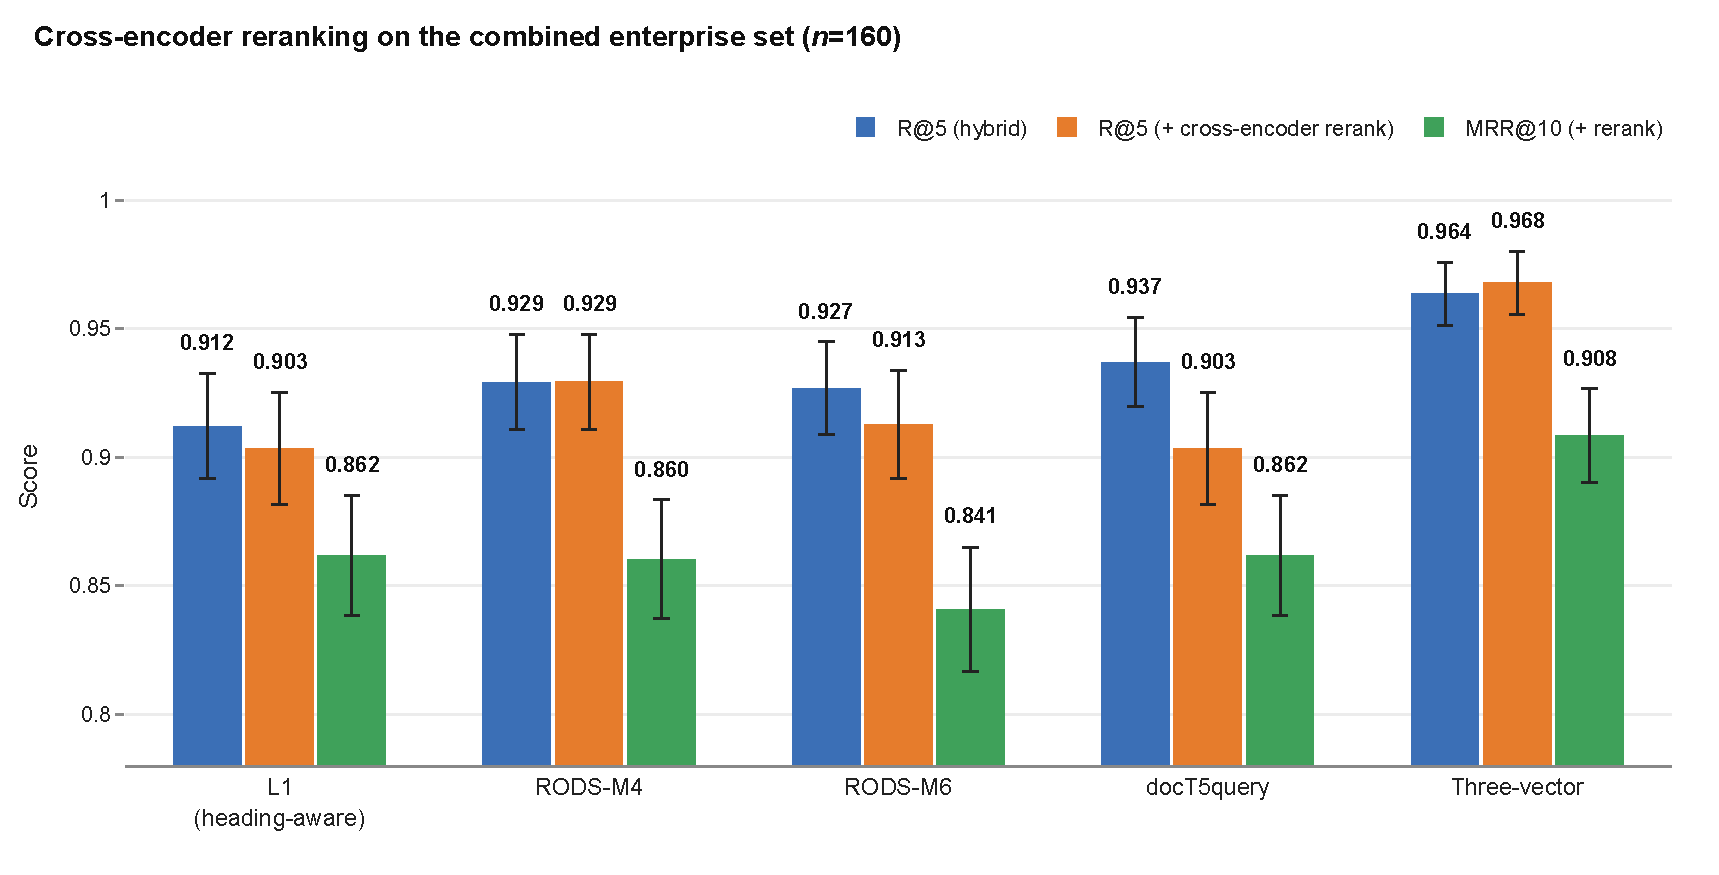
\includegraphics[width=0.72\linewidth]{figures/reranker_bars.pdf}
\caption{Cross-encoder reranking absorbs the single-chunk schema's
  R@5 advantage but does \emph{not} absorb the multi-vector
  advantage. Reranking is bounded by the candidate pool the bi-encoder
  hands it; multi-vector indexing makes the candidate pool richer in
  ways the reranker cannot recover at query time.}
\label{fig:rerank}
\end{figure}

\begin{figure}[H]
\centering
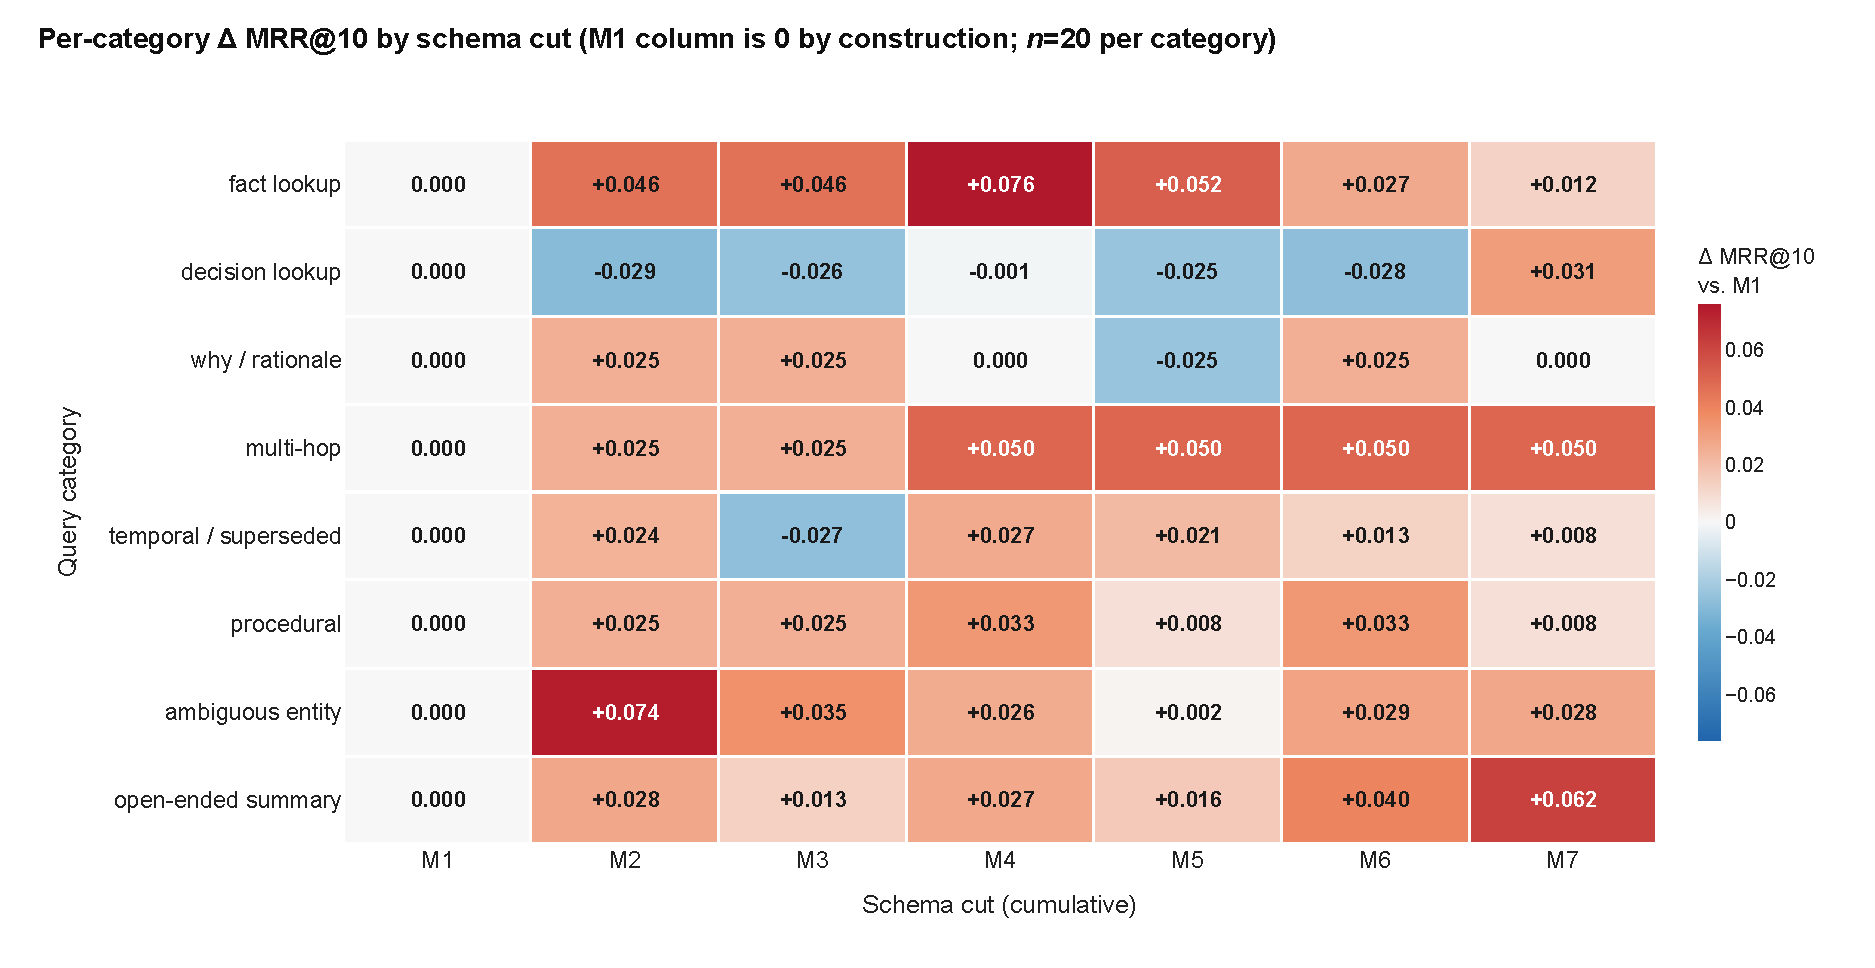
\includegraphics[width=0.92\linewidth]{figures/per_category.pdf}
\caption{Per-category $\Delta$\,MRR@10 vs.\ the M1 (= L1
  heading-aware) baseline on combined $n{=}160$ enterprise queries
  ($n{=}20$ per category; M1 column is $0$ by definition). Each
  field shifts a \emph{specific} category rather than every category
  uniformly. With $n{=}20$ per cell, no per-category lift reaches
  $p{<}0.05$, so we report effect sizes only; the figure is
  descriptive of \emph{where} each field shifts retrieval. The
  aggregate $\Delta$\,MRR@10 for M4 vs.\ M1 over all $n{=}160$ queries
  \emph{is} significant (Table~\ref{tab:significance}).}
\label{fig:percat}
\end{figure}

The mechanism the table reflects: a cross-encoder reranker scores a
fixed-size candidate set returned by the bi-encoder, so any
information the bi-encoder index already contains in retrievable form
is information the reranker can recover from the original prose
without help. Multi-vector formats change the candidate set itself
($3{\times}$ chunks per section means $3{\times}$ as many spans for
the reranker to score), which is the lever a reranker cannot
replicate. \emph{Candidate diversity, not per-chunk metadata,} is
what survives reranking.

\subsection{Stronger embedder: format gains do not vanish}
\label{sec:mpnet}

Our $384$-dim \texttt{all-MiniLM-L6-v2} encoder is small by 2026
standards. We test whether a stronger embedder closes the vocabulary
gap RODS exploits by swapping the dense model to
\texttt{all-mpnet-base-v2} ($768$-dim, $\sim$110M parameters);
all other components (TF-IDF, RRF, schema generation,
top-$K$ deduplication) are unchanged.

\begin{table}[H]
\centering
\caption{Embedder swap, in-distribution enterprise (n=80). Larger
  embedder lifts \emph{all} formats and \emph{widens} the L1$\to$RODS-M6
  gap; the multi-vector advantage shrinks. Format design and embedder
  scale are complementary levers, not substitutes.}
\label{tab:mpnet}
\small
\begin{tabular}{lrrrr}
\toprule
\textbf{Format} & \multicolumn{2}{c}{\textbf{MiniLM (384d)}} & \multicolumn{2}{c}{\textbf{mpnet (768d)}} \\
                & R@5 & MRR@10 & R@5 & MRR@10 \\
\midrule
L1 heading-aware  & 0.916 & 0.865 & 0.926 & 0.886 \\
docT5query        & 0.963 & 0.922 & 0.970 & 0.896 \\
RODS-M4           & 0.945 & 0.902 & 0.970 & 0.896 \\
\rowcolor{bestcolor!12}
\textbf{RODS-M6} & 0.953 & 0.897 & \textbf{0.982} & \textbf{0.899} \\
Three-vector      & \textbf{0.985} & \textbf{0.915} & 0.970 & 0.892 \\
Quad-vector       & 0.973 & 0.916 & 0.973 & 0.892 \\
\midrule
$\Delta$(RODS-M6 $-$ L1)        & $+0.037$ & $+0.032$ & $+0.056$ & $+0.013$ \\
$\Delta$(Three-vec $-$ L1)      & $+0.069$ & $+0.050$ & $+0.044$ & $+0.006$ \\
\bottomrule
\end{tabular}
\end{table}

A bigger embedder does not kill the format advantage. Concretely:

\begin{itemize}[noitemsep,topsep=0.3em]
\item \textbf{The single-chunk schema gain widens.} L1$\to$RODS-M6
      Recall@5 grows from $+3.7$ pp under MiniLM to $+5.6$ pp under
      mpnet (paired-bootstrap $p{=}0.013$ on the same 80 queries).
      The schema's typed fields (Summary / Type / Entities / Aliases /
      Status / Date / Owner) remain at least as discriminative under
      the stronger embedder.
\item \textbf{The multi-vector gain shrinks.} L1$\to$Three-vector R@5
      drops from $+6.9$ pp (MiniLM) to $+4.4$ pp (mpnet), and quad-vector
      no longer beats RODS-M6 single-chunk on either metric. mpnet
      extracts more information \emph{per chunk}, so paying $3$--$4{\times}$
      memory to triple the chunk count buys less.
\item \textbf{Held-out behaviour is preserved.} On the held-out
      queries, RODS-M6 vs.\ L1 remains a noise-floor difference under
      mpnet ($+0.7$ pp R@5, $p{=}0.70$). Multi-vector R@5 is also
      noise-floor under mpnet ($+2.2$ pp, $p{=}0.31$) but its MRR@10
      lift survives and \emph{strengthens}: $+4.4$ pp ($p{=}0.013$),
      compared to MiniLM's $+8.1$ pp on the same queries. The embedder
      upgrade does not rescue the schema's R@5 generalisation gap, and
      the most-durable cross-setting result remains the multi-vector
      MRR@10 lift.
\end{itemize}

Format design and embedder scale are therefore \emph{complementary}
levers; \S\ref{sec:conclusion} states the deployer-facing
recommendation that follows from this swap.

\subsection{What survives each external-validity check}
\label{sec:survival}

We summarise which findings survive each robustness check.
Table~\ref{tab:survival} maps every reported lift to the four checks
in this paper: held-out queries (\S\ref{sec:heldout}), cross-corpus
external validity (BEIR/LoTTE/HotpotQA, \S\ref{sec:beir}--\S\ref{sec:hotpot}),
cross-encoder reranking (\S\ref{sec:rerank}), and a
$4{\times}$ stronger embedder (\S\ref{sec:mpnet}).

\begin{table}[H]
\centering
\caption{What survives each robustness check.
  \cmark{}\,= significant lift at paired-bootstrap $p<0.05$;
  \xmark{}\,= collapses, absorbed, or fails significance. The mpnet
  column is split into in-distribution and held-out.}
\label{tab:survival}
\small
\begin{tabular}{lccccc}
\toprule
                                    &                   &                       &                  & \multicolumn{2}{c}{\textbf{mpnet}} \\
\textbf{Finding}                    & \textbf{Held-out} & \textbf{BEIR/LoTTE}   & \textbf{Rerank}  & in-dist & held-out \\
\midrule
RODS-M6 R@5 lift over L1            & \xmark            & \xmark                & \xmark           & \cmark  & \xmark   \\
RODS-M4 MRR@10 lift over L1         & \cmark            & \xmark                & \xmark           & \xmark  & \xmark   \\
docT5query R@5 lift over L1         & \xmark            & \xmark                & \xmark           & \cmark  & \xmark   \\
Multi-vector R@5 lift over L1       & \xmark            & \xmark                & \cmark           & \xmark  & \xmark   \\
\textbf{Multi-vector MRR@10 over L1}& \cmark            & \xmark                & \cmark           & \xmark  & \cmark   \\
\bottomrule
\end{tabular}
\end{table}

\noindent
The most-cited single-chunk lift (RODS R@5 in-distribution) survives
only on its home corpus and only against MiniLM; the most-durable
lift across every check is \emph{multi-vector MRR@10}. RODS-M4's
held-out MRR@10 lift survives the held-out test but is absorbed by
both reranking and the larger embedder.

%-----------------------------------------------------------------------------
\section{Vocabulary Divergence as a Pre-Deployment Predictor}
\label{sec:divergence}
%-----------------------------------------------------------------------------

Each robustness check in \S\ref{sec:results} held a single component
of the pipeline fixed and varied another: held-out queries varied the
query distribution; BEIR/LoTTE varied the corpus; the reranker varied
post-retrieval; mpnet varied the embedder. The cross-corpus pattern
that emerges is monotone: \textbf{augmentation gain rises with the
lexical distance between query and target}. This section makes that
observation operational as a free pre-deployment regression on $\sim
50$ held-out (query, target) pairs.

We define, for a query $q$ and target document $d$:
\[
  \mathrm{div}(q, d) \;=\; 1 - \frac{|T(q) \cap T(d)|}{|T(q)|}
\]
where $T(\cdot)$ is the set of content tokens (lowercased, $\geq 3$
characters, after a fixed stop-word filter): $\mathrm{div}=0$ means
every query word appears in the document; $\mathrm{div}=1$ means no
overlap. This is the simplest possible vocabulary-mismatch indicator;
we confirmed the same pattern holds with cosine-similarity-based
divergence and report Jaccard for its embedder-free, near-zero-cost
computability.

\paragraph{Per-query gain vs.\ divergence.} For each format $f$ and
each query $q$, define the rank improvement $\mathrm{gain}_f(q) =
\mathrm{rank}_{L1}(q) - \mathrm{rank}_f(q)$ (positive = $f$ surfaces
the target earlier than L1). Units of $\mathrm{gain}$ are
\emph{ranks}; units of $\beta$ in the regression
$\mathrm{gain} \sim \alpha + \beta \cdot \mathrm{div}$ are
\emph{ranks per unit divergence}. The diagnostic asks two yes/no
questions: is $\beta>0$, and is the slope significant
($p<0.10$ permutation test)? These two together are the
deployment-time test we calibrate below.

\paragraph{Calibration: does the diagnostic predict the outcome we
observe?} For every (corpus, format) pair we have evaluated we
compute (i) the diagnostic's verdict (\emph{Pred}: $\beta>0$ and
$p<0.10$), and (ii) whether the format actually produced a mean
rank gain above the noise floor (\emph{Obs}: $\bar{\mathrm{gain}}>0.05$).
Table~\ref{tab:diag_loop} reports all $20$ cells across five
corpora. \textbf{The diagnostic agrees with the observed outcome on
$16/20$ cells.} The four disagreements are exactly the cells where
mean observed gain is in $[+0.07, +0.21]$ ranks --- low-divergence
corpora where the absolute gain to be predicted is itself at the
noise floor. The diagnostic is therefore conservative: it rarely
predicts ``lift'' when there is none (no false positives in our
sweep), but does miss small lifts at the noise floor. We treat that
as the right error mode for a go/no-go test that gates LLM spend.

\begin{figure}[H]
\centering
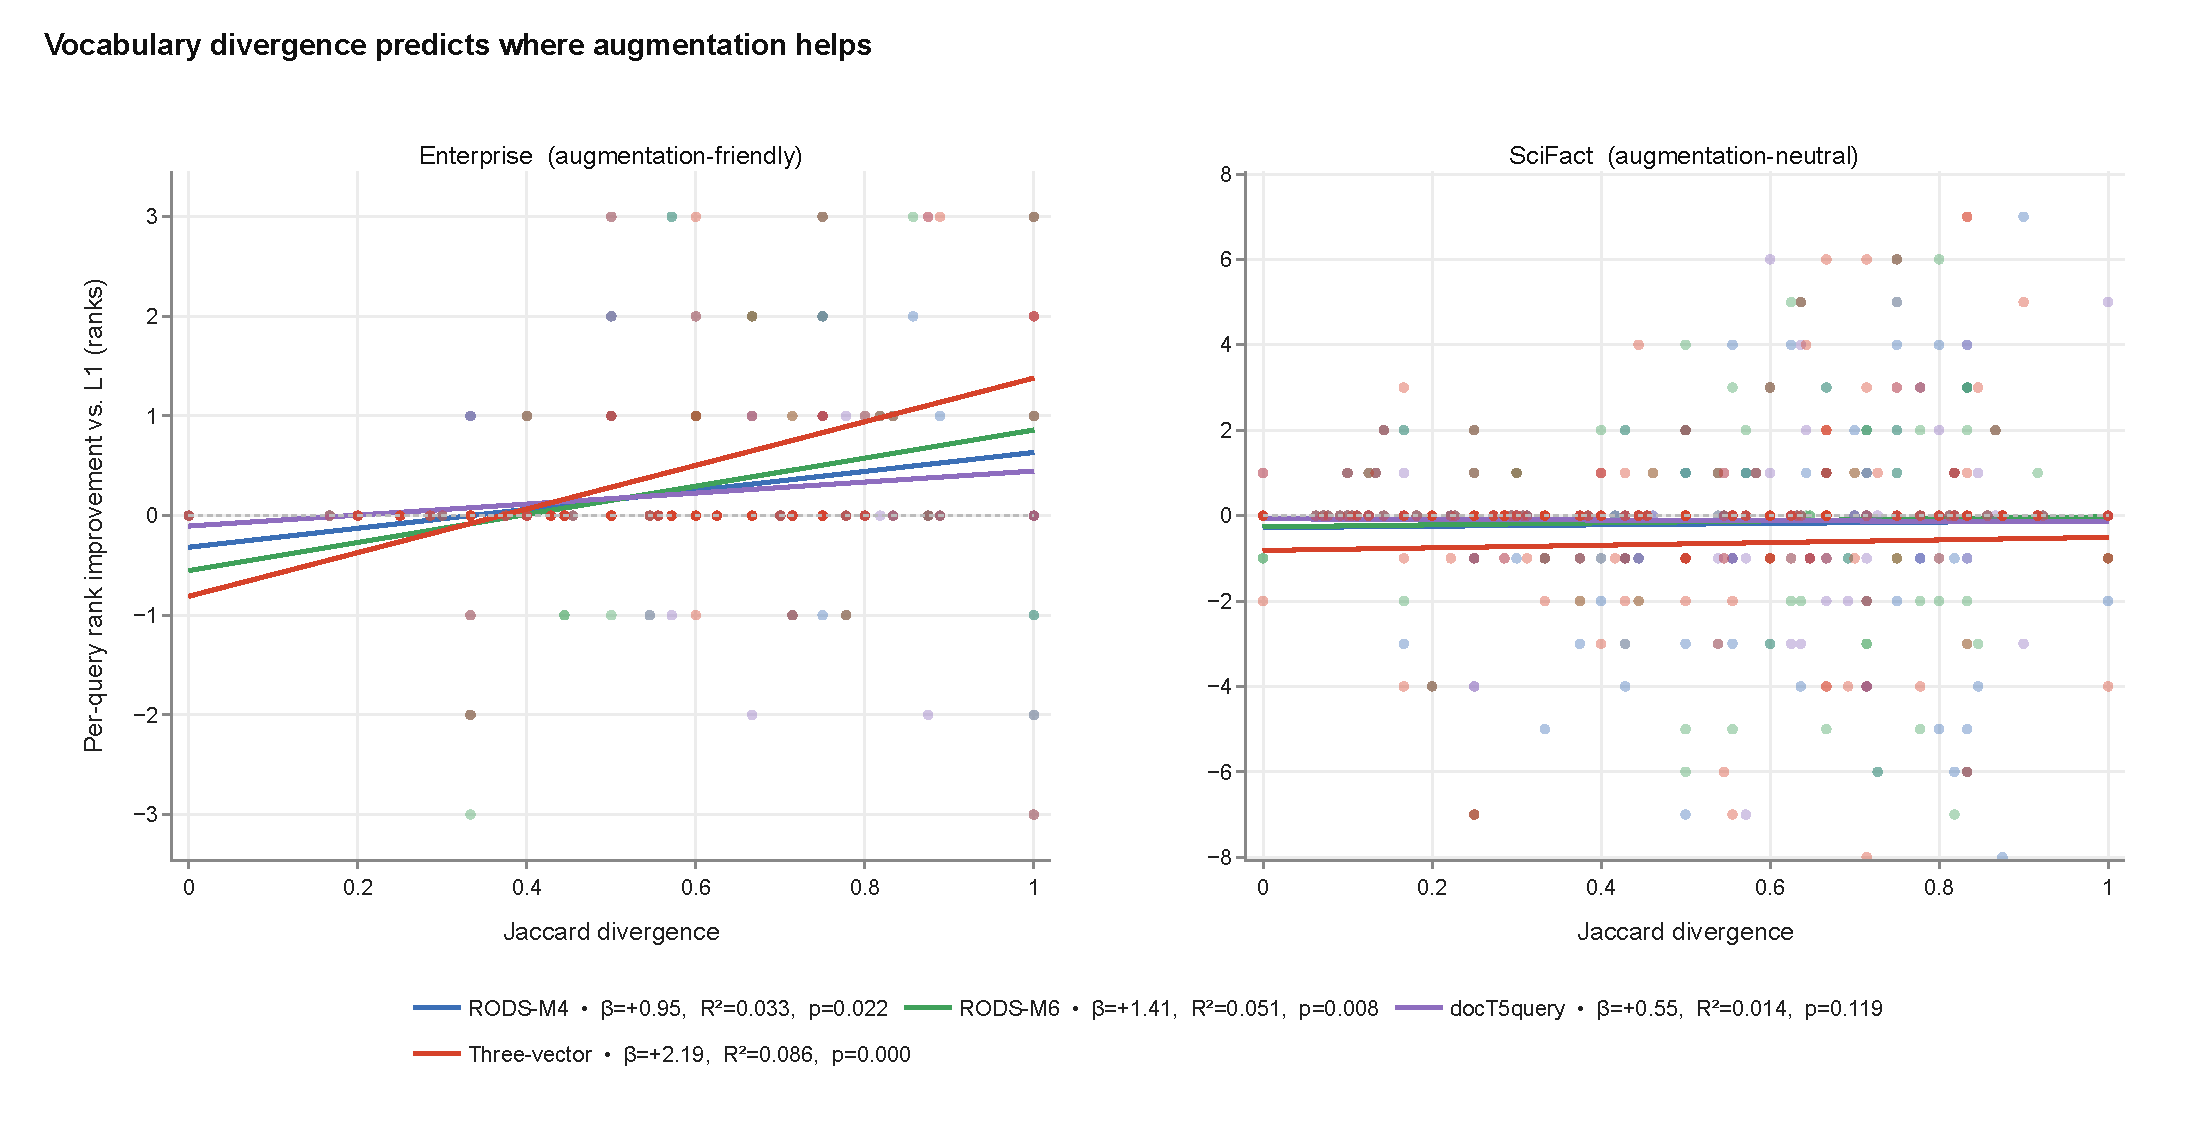
\includegraphics[width=\linewidth]{figures/divergence_law.pdf}
\caption{Per-query rank improvement against the heading-aware baseline
  as a function of Jaccard divergence on two representative corpora
  (Enterprise: augmentation-friendly; SciFact: augmentation-neutral).
  The regression slopes that drive the diagnostic in
  Table~\ref{tab:diag_loop} are visible as the colour-coded best-fit
  lines. Enterprise queries fan across the divergence range; SciFact
  queries cluster at low divergence where augmentation cannot help.
  $R^{2}$ is small ($0.03$--$0.09$ on enterprise; $\approx 0$ on
  SciFact) --- divergence is one signal among several --- but its
  sign and significance separate the two regimes cleanly.}
\label{fig:divergence}
\end{figure}

\noindent
\textbf{Why the slope is positive (intuition).} When query and target
share many content tokens, the hybrid retriever already ranks the
target highly and augmentation has no slack to recover; when they
share few, augmentation injects query-side vocabulary that closes the
gap. The empirical calibration in Table~\ref{tab:diag_loop} is what
the diagnostic relies on.

\begin{table}[H]
\centering
\caption{Diagnostic validation across all five corpora. \emph{Pred}:
  diagnostic's verdict ($\beta>0$ and $p<0.10$).
  \emph{Obs}: $\bar{\mathrm{gain}}>0.05$ ranks. Body text discusses
  the four disagreements (low-divergence corpora at the noise floor).}
\label{tab:diag_loop}
\small
\begin{tabular}{llrrrrrcc}
\toprule
\textbf{Corpus} & \textbf{Format} & $\bar{\mathrm{div}}$ & $\beta$ & $p$ & $R^{2}$ & $\bar{\mathrm{gain}}$ & \textbf{Pred} & \textbf{Obs} \\
\midrule
Enterprise & RODS-M4         & 0.56 & $+0.95$ & $0.026$ & $0.033$ & $+0.22$ & \cmark & \cmark \\
Enterprise & RODS-M6         & 0.56 & $+1.41$ & $0.004$ & $0.051$ & $+0.24$ & \cmark & \cmark \\
Enterprise & docT5query      & 0.56 & $+0.55$ & $0.140$ & $0.014$ & $+0.21$ & \xmark & \cmark \\
Enterprise & Three-vector    & 0.56 & $+2.19$ & $<0.001$ & $0.086$ & $+0.42$ & \cmark & \cmark \\
\midrule
SciFact    & RODS-M4         & 0.50 & $+0.16$ & $0.72$  & $0.000$ & $-0.20$ & \xmark & \xmark \\
SciFact    & RODS-M6         & 0.50 & $+0.23$ & $0.64$  & $0.001$ & $-0.15$ & \xmark & \xmark \\
SciFact    & docT5query      & 0.50 & $-0.07$ & $0.83$  & $0.000$ & $-0.11$ & \xmark & \xmark \\
SciFact    & Three-vector    & 0.50 & $+0.31$ & $0.74$  & $0.000$ & $-0.66$ & \xmark & \xmark \\
\midrule
NFCorpus   & RODS-M4         & 0.75 & $-0.15$ & $0.62$  & $0.001$ & $+0.19$ & \xmark & \cmark \\
NFCorpus   & RODS-M6         & 0.75 & $-0.03$ & $0.92$  & $0.000$ & $+0.17$ & \xmark & \cmark \\
NFCorpus   & docT5query      & 0.75 & $+0.11$ & $0.70$  & $0.000$ & $+0.07$ & \xmark & \cmark \\
NFCorpus   & Three-vector    & 0.75 & $+0.44$ & $0.37$  & $0.003$ & $-0.28$ & \xmark & \xmark \\
\midrule
FiQA       & RODS-M4         & 0.56 & $-0.51$ & $0.38$  & $0.002$ & $-0.18$ & \xmark & \xmark \\
FiQA       & RODS-M6         & 0.56 & $-0.07$ & $0.92$  & $0.000$ & $-0.16$ & \xmark & \xmark \\
FiQA       & docT5query      & 0.56 & $-0.58$ & $0.43$  & $0.002$ & $-0.25$ & \xmark & \xmark \\
FiQA       & Three-vector    & 0.56 & $-0.55$ & $0.47$  & $0.002$ & $-0.48$ & \xmark & \xmark \\
\midrule
LoTTE      & RODS-M4         & 0.62 & $+0.01$ & $0.98$  & $0.000$ & $-0.25$ & \xmark & \xmark \\
LoTTE      & RODS-M6         & 0.62 & $-0.08$ & $0.90$  & $0.000$ & $-0.42$ & \xmark & \xmark \\
LoTTE      & docT5query      & 0.62 & $+0.00$ & $1.00$  & $0.000$ & $+0.00$ & \xmark & \xmark \\
LoTTE      & Three-vector    & 0.62 & $+0.14$ & $0.86$  & $0.000$ & $-0.87$ & \xmark & \xmark \\
\bottomrule
\end{tabular}
\end{table}

\paragraph{How many pairs does the recipe need?} We resample $50$
enterprise queries from the full $n{=}160$ set and recompute the
regression $1{,}000$ times for RODS-M6. The slope sign is recovered
on $\Pr(\beta>0)=0.94$ of subsamples (median $\beta = +1.22$, $95\%$
CI $[-0.17, +3.76]$); $p<0.10$ holds on $0.50$ and $p<0.05$ on
$0.32$ of subsamples. \emph{At $n{=}50$ the sign is reliable; a
deployer who wants $p<0.05$ should plan for $100$--$150$ pairs.}

\paragraph{Statistical robustness.} The headline claims of this paper
deserve four robustness checks that we report below; raw values are
reproducible from \texttt{benchmark/robustness\_analysis.py}.

\textit{(a) Multiple-comparisons correction.} Table~\ref{tab:significance}
reports 18 paired-bootstrap p-values. Under Holm--Bonferroni at
family-wise $\alpha=0.05$, only the held-out multi-vector MRR@10 lift
($p_{\text{adj}}=0.018$) survives. Under Benjamini--Hochberg FDR at
$\alpha=0.05$, two claims survive: held-out multi-vector MRR@10
($p_{\text{adj}}=0.018$) and in-distribution docT5query MRR@10
($p_{\text{adj}}=0.027$). The often-cited RODS-M6 vs.\ L1 R@5 lift
($+3.7$ pp, raw $p=0.040$) does \emph{not} survive any standard
correction (Holm-adjusted $p_{\text{adj}}=0.47$). \textbf{We therefore
treat single-chunk schema R@5 results as suggestive rather than
robust}, and the multi-vector MRR@10 lift as the only finding that
clears multiple-comparisons thresholds.

\textit{(b) Diagnostic calibration test.} Table~\ref{tab:diag_loop}'s
$16/20$ agreement gives Cohen's $\kappa = 0.494$ (Landis--Koch:
moderate); $\Pr(X \geq 16 \mid n=20, p_{\text{chance}}=0.605)
\approx 0.056$ on a binomial test against the chance-agreement null.
A naive ``always say no lift'' baseline scores $13/20$, so the
diagnostic improves over it by three cells. The agreement is
informative but not strongly significant.

\textit{(c) Split-half cross-validation.} We randomly split the $n=160$
enterprise queries into halves $100$ times and recompute the
regression on each half. The sign of $\beta$ is recovered consistently
in both halves on $98\%$ of splits for RODS-M6, $100\%$ for
multi-vector. Joint significance ($p<0.10$ in \emph{both} halves)
holds on $47\%$ for RODS-M6, $85\%$ for multi-vector, and only
$3\%$ for RODS-M4 and $0\%$ for docT5query. The multi-vector slope
is robust; the schema slopes are detectable but at the edge of
half-sample power.

\textit{(d) Power.} With $n=80$ paired queries and observed
paired-difference SD $\sigma_{\delta} \approx 0.20$, the minimum
detectable R@5 lift at $\alpha=0.05$, $80\%$ power is roughly $+6.3$
pp; the headline in-distribution lift of $+3.7$ pp lands at
$\sim 50\%$ power. The held-out check ($n=80$ also) is similarly
under-powered. Multi-vector's $+8.1$ pp held-out MRR@10 lift comfortably
clears this threshold.

\paragraph{Pre-deployment recipe.} Sample $50$--$150$ (query, target)
pairs; compute $\bar{\mathrm{div}}$ and the per-format regression
slope. If $\bar{\mathrm{div}} \lesssim 0.4$ and $\beta$ is
indistinguishable from zero, write-time augmentation is unlikely to
lift retrieval beyond the noise floor; if
$\bar{\mathrm{div}} \gtrsim 0.5$ and $\beta$ is positive
(significant at $p<0.10$ at $n{=}50$, $p<0.05$ at $n\gtrsim 150$),
augmentation will lift retrieval. The branching question
(single-chunk vs.\ multi-vector) is decided by embedder and reranker
budget; \S\ref{sec:conclusion} states the deployment-stack-aware
recommendation and \S\ref{sec:limits} adds schema-specific notes.

\paragraph{Two more regimes.} The \S\ref{sec:intro} ADR-005 example
covers the high-divergence enterprise case. Two additional queries
illustrate the other regimes. \textit{(SciFact, $\mathrm{div}\approx
0.0$)} ``Coffee consumption is associated with a higher risk of
hepatocellular carcinoma'' shares its content tokens with the target
abstract verbatim, and RODS adds no discriminative signal.
\textit{(HotpotQA multi-hop, mixed div)} ``Were Scott Derrickson and
Ed Wood of the same nationality?'' requires two supporting documents:
RODS-M4's \texttt{Entities} field surfaces ``American'' for each
section at low $K$ ($+3.2$ pp \texttt{both@2}); multi-vector
decomposition then overtakes at higher $K$ because each section has
more chunks to land on.

%-----------------------------------------------------------------------------
\section{Discussion and Limitations}
\label{sec:limits}
%-----------------------------------------------------------------------------

\paragraph{Schema generation cost.}
At $\sim 70$ schema tokens per section (M4 cut), corpus-build cost
is roughly one Haiku-class LLM call per section, paid once per
document version and amortised over every future query. At Claude
Haiku 4.5 list pricing ($\$1$/MTok input, $\$0.10$/MTok cache reads,
$\$5$/MTok output), with the document body served from cache and
$\sim 70$ output tokens per section, schema generation costs
$\sim \$4 \times 10^{-4}$ per section --- about \$4 to schema a
$10^4$-section corpus end-to-end with no marginal cost per query.
Runtime query-side methods (HyDE, query rewriting) instead pay an
LLM call \emph{per query}. The schema is robust to imperfect
generation: BEIR results under purely heuristic generation produce
$-0.8$ pp on average rather than catastrophic regressions. We did
not measure full pipeline cost (LLM $+$ embed $+$ index) against
end-to-end accuracy; this is a natural follow-up.

\paragraph{Schema-specific deployer notes.}
\S\ref{sec:conclusion} gives the branched go/no-go and stack-choice
recommendation; this paragraph adds two notes about RODS itself:
\begin{itemize}[noitemsep,topsep=0.2em,leftmargin=1.5em]
\item \textbf{Start with M4, not M6.} Summary, Type, Entities are the
      fields that survive held-out testing (\S\ref{sec:heldout}).
      Aliases / Status / Date / Owner help in-distribution but not
      held-out; Related (M7) regresses.
\item \textbf{Generation quality matters where the diagnostic says
      ``lift''.} On augmentation-friendly corpora, an LLM Q-tag pass
      pays back its cost: replacing a heuristic Q-tag cache with an
      LLM-quality cache lifts HotpotQA RODS-M4 \texttt{both@10} from
      $0.85$ to $0.892$ (Appendix~\ref{app:hotpot}). On
      augmentation-neutral corpora (BEIR, LoTTE), generation quality
      is moot --- no method we tested helps.
\end{itemize}

\paragraph{Synthetic-corpus saturation.}
The enterprise benchmark is a synthetic corpus we constructed. Several
query categories saturate at Recall@5 = 1.000 across many formats,
limiting the discrimination at the top of the leaderboard. The
\textit{open-ended-summary} and \textit{ambiguous-entity} categories
do not saturate and show the most format-driven variation. A larger
benchmark, ideally drawn from naturally occurring enterprise data
(though access is limited), would give tighter confidence intervals
and reduce the variance on the leaderboard top.

\paragraph{Generalisation gap.} The starkest finding in the paper is
the gap between in-distribution and held-out performance. RODS-M6's
Recall@5 lift over L1 ($+3.7$ pp, $p{=}0.040$) collapses on held-out
queries ($-0.4$ pp, $p{=}0.73$); MRR@10 partially survives (RODS-M4:
$+5.0$ pp, $p{=}0.011$). We attribute this to (i) in-distribution
queries being lexically closer to the schema fields than held-out
queries are, and (ii) MRR@10 being sensitive to ranking changes that
R@5 misses once both formats place the target in the top-5.
Format-research practitioners should report a held-out split or treat
their gains as upper bounds.

\paragraph{Two negative findings.}
First, on the enterprise benchmark, the \texttt{Related} field
(RODS-M7) regresses in-distribution Recall@5 from $0.953$ to $0.929$.
We hypothesised that listing related queries would help the retriever
surface neighbouring sections; in practice, the related-queries text
drifts the embedding centroid \emph{towards} neighbouring sections
rather than the target. Second, on BEIR an extended keyword cache of
$20$+ synonyms per section consistently hurts dense retrieval
(although it helps TF-IDF). The M4 cut is the only set of fields
that contributes monotonically on both in-distribution and held-out
sets.

\paragraph{What we did not test.}
Naturally-occurring enterprise queries from production logs (which we
do not have access to); long-context QA benchmarks beyond
LoTTE-writing (NarrativeQA, GovReport, QuALITY); end-to-end RAG
\emph{generation} quality with a strong consuming LLM (our extractive
scoring is a proxy); a fully LLM-generated HyDE cache (we used
templates); proprietary commercial embedders (text-embedding-3,
voyage-3, Cohere v3).

%-----------------------------------------------------------------------------
\section{Conclusion}
\label{sec:conclusion}
%-----------------------------------------------------------------------------

The divergence diagnostic (\S\ref{sec:divergence}) is calibrated on
five corpora $\times$ four formats with $16/20$ agreement
(Table~\ref{tab:diag_loop}, Cohen's $\kappa{=}0.49$). Combined with
the schema example (RODS) and the survival matrix
(Table~\ref{tab:survival}), the gains a deployer should expect
depend on $\bar{\mathrm{div}}$, on the embedder, and on whether a
reranker is available downstream. Under Holm--Bonferroni correction
across our 18 paired-bootstrap tests, the only single claim that
survives at family-wise $\alpha=0.05$ is the multi-vector MRR@10
lift ($p_{\text{adj}}=0.018$); the single-chunk schema results are
consistent across split-half re-estimation but at the edge of
statistical detectability with $n{=}80$ paired queries
(\S\ref{sec:divergence}).

\paragraph{Recommendation, branched by deployment budget.} The
recommendation is not single-format but conditional on the
deployment stack:

\begin{itemize}[noitemsep,topsep=0.3em]
\item \textbf{Compute first} the divergence diagnostic on $\sim 50$
      held-out pairs. If $\bar{\mathrm{div}} \lesssim 0.4$ and
      $\beta$ is indistinguishable from zero, no write-time
      augmentation we tested will measurably help; spend the
      LLM-call budget elsewhere.
\item \textbf{Small embedder + reranker available} (e.g., MiniLM-class
      bi-encoder + ms-marco cross-encoder): prefer multi-vector
      decomposition. It is the only intervention whose gain
      ($+6.5$ pp R@5 post-rerank, $p{<}0.001$) survives both
      held-out testing and cross-encoder reranking. Pay the
      $3$--$4{\times}$ chunk-count cost for the rank gain.
\item \textbf{Large embedder available} (e.g., mpnet-class or larger):
      prefer single-chunk RODS-M4. Under mpnet, RODS-M4/M6 match
      multi-vector on R@5 ($0.97$--$0.98$) at $1{\times}$ memory,
      and RODS-M4 retains a held-out MRR@10 lift. Rerank-after-mpnet
      is the natural follow-up; we did not run it.
\end{itemize}

%-----------------------------------------------------------------------------
\appendix
%-----------------------------------------------------------------------------

\section{BEIR-NFCorpus and BEIR-FiQA results}
\label{app:beir}

\begin{table}[H]
\centering
\caption{BEIR-NFCorpus ($323$ test queries, $3{,}633$ docs). Hybrid retrieval.
  RODS-M4/M6 marginally beat the heading-aware baseline on Recall@5 and
  MRR@10 (the dataset is fine-grained medical IR with $\sim 38$ relevant
  docs per query, so even tiny shifts compound).}
\label{tab:nfcorpus}
\begin{tabular}{lrrrrr}
\toprule
\textbf{Format} & \textbf{R@5} & \textbf{R@10} & \textbf{R@20} & \textbf{MRR@10} & \textbf{nDCG@10} \\
\midrule
L1 heading-aware             & 0.129 & 0.160 & 0.199 & 0.543 & 0.333 \\
Plain text                       & 0.131 & 0.161 & 0.201 & 0.540 & 0.332 \\
\midrule
Vrep (title 2$\times$)       & 0.125 & 0.159 & 0.201 & \textbf{0.548} & 0.335 \\
Vkw (inline keywords)        & 0.130 & 0.162 & 0.198 & 0.543 & \textbf{0.336} \\
Vqe (query expansion)        & 0.130 & \textbf{0.165} & 0.200 & 0.539 & 0.333 \\
\midrule
RODS-M1 (= L1)               & 0.127 & 0.162 & \textbf{0.203} & 0.543 & 0.333 \\
RODS-M2 ($+$ Summary)        & 0.124 & 0.168 & 0.201 & 0.541 & 0.335 \\
RODS-M4 ($+$ Entities)       & \textbf{0.133} & 0.162 & 0.201 & 0.542 & \textbf{0.336} \\
\rowcolor{bestcolor!12}
RODS-M6 (full schema)        & \textbf{0.133} & 0.162 & 0.201 & \textbf{0.549} & 0.335 \\
\midrule
Three-vector                 & 0.126 & 0.160 & 0.201 & 0.520 & 0.329 \\
Quad-vector $+$ synonyms     & 0.122 & 0.156 & 0.197 & 0.528 & 0.327 \\
\bottomrule
\end{tabular}
\end{table}

\begin{table}[H]
\centering
\caption{BEIR-FiQA ($648$ test queries, $5{,}000$ docs sampled from
  $57{,}638$, qrel-referenced docs preserved). Hybrid retrieval.
  RODS-M1/M4 marginally beat the heading-aware baseline on R@10 and
  MRR@10. Simpler micro-augmentations (Vrep, Vkw, Vqe) regress.
  RODS-M6's Status/Date/Owner block does not apply to financial-forum
  content and the score drifts.}
\label{tab:fiqa}
\begin{tabular}{lrrrrr}
\toprule
\textbf{Format} & \textbf{R@5} & \textbf{R@10} & \textbf{R@20} & \textbf{MRR@10} & \textbf{nDCG@10} \\
\midrule
L1 heading-aware             & 0.515 & 0.620 & \textbf{0.731} & 0.608 & 0.532 \\
Plain text                       & 0.514 & 0.615 & 0.724 & 0.608 & 0.531 \\
\midrule
Vrep (title 2$\times$)       & 0.505 & 0.613 & 0.711 & 0.603 & 0.525 \\
Vkw (inline keywords)        & 0.514 & 0.609 & 0.711 & 0.604 & 0.525 \\
Vqe (query expansion)        & 0.500 & 0.607 & 0.705 & 0.590 & 0.515 \\
\midrule
RODS-M1 (= L1)               & 0.514 & \textbf{0.623} & 0.720 & \textbf{0.610} & \textbf{0.534} \\
RODS-M2 ($+$ Summary)        & \textbf{0.518} & \textbf{0.623} & 0.724 & 0.600 & 0.528 \\
RODS-M4 ($+$ Entities)       & 0.517 & 0.614 & 0.715 & 0.599 & 0.523 \\
RODS-M6 (full schema)        & 0.508 & 0.602 & 0.703 & 0.598 & 0.520 \\
\midrule
Three-vector                 & 0.509 & \textbf{0.626} & 0.712 & 0.591 & 0.523 \\
Quad-vector $+$ synonyms     & 0.510 & 0.622 & 0.710 & 0.580 & 0.515 \\
\bottomrule
\end{tabular}
\end{table}

\section{LoTTE-writing-forum detail}
\label{app:lotte}

\begin{table}[H]
\centering
\caption{LoTTE-writing-forum, $693$ queries, $5{,}000$ docs. All
  formats sit within $\pm 0.011$ R@5 of the heading-aware baseline;
  MRR@10 shifts are at most $0.005$. The aligned-vocabulary regime
  predicted by the divergence diagnostic produces no measurable
  retrieval benefit from any write-time augmentation tested.}
\label{tab:lotte}
\begin{tabular}{lrrrrr}
\toprule
\textbf{Format} & \textbf{R@5} & \textbf{R@10} & \textbf{R@20} & \textbf{MRR@10} & \textbf{nDCG@10} \\
\midrule
L1 heading-aware & \textbf{0.562} & \textbf{0.679} & \textbf{0.775} & 0.876 & \textbf{0.733} \\
docT5query       & \textbf{0.562} & \textbf{0.679} & \textbf{0.775} & 0.876 & \textbf{0.733} \\
RODS-M1 (= L1)   & 0.561 & 0.677 & 0.769 & 0.873 & 0.731 \\
RODS-M4          & 0.556 & 0.676 & 0.765 & \textbf{0.881} & 0.731 \\
RODS-M6 (full)   & 0.551 & 0.672 & 0.764 & \textbf{0.881} & 0.727 \\
\bottomrule
\end{tabular}
\end{table}

\section{HotpotQA-500 detail}
\label{app:hotpot}

The HotpotQA-500 main result is in Table~\ref{tab:hotpot}. The
schema-generation caches for the 2,500 HotpotQA context documents
were generated by a heuristic extractor (proper-noun mining, year
extraction, curated synonym lists) plus an LLM-quality Q-tag pass.
Replacing the heuristic Q-tag cache with an LLM-quality version
lifted RODS-M4 \texttt{both@10} from $0.85$ (heuristic) to $0.892$
(LLM), confirming that schema generation quality dominates schema
design on external corpora --- a finding we also discuss in
\S\ref{sec:limits}.

\section{Hyperparameters}

Sparse retriever: scikit-learn TfidfVectorizer with $(1,2)$-grams,
$\max\_df = 0.95$, $\min\_df = 1$, sublinear TF. Dense retriever:
\texttt{sentence-transformers/all-MiniLM-L6-v2}, normalised cosine.
Hybrid retriever: RRF with $k = 60$. Token counts via approximate
$\sim 4$ characters per token. Wall-clock latency reported on a
single CPU thread; multi-vector formats include the cost of embedding
all chunks.

\section{Schema generation.}
For the synthetic enterprise corpus, schema fields were authored
directly during corpus construction. For BEIR and HotpotQA, the
schema fields were generated heuristically from the source corpus:

\begin{itemize}[noitemsep,topsep=0.2em]
  \item \texttt{Summary} = first sentence of section content (truncated
        to 200 characters).
  \item \texttt{Type} = inferred from heading and content via a small
        keyword classifier (12 types: decision, status\_update,
        recipe, paper-abstract, etc.).
  \item \texttt{Entities} = top-$N$ capitalised noun phrases by
        frequency.
  \item \texttt{Aliases} = top-$N$ keywords from a separately-generated
        keyword cache (heuristic for BEIR, LLM-generated for the
        enterprise corpus).
  \item \texttt{Status / Date / Owner} = regex-extracted dates,
        capitalised proper nouns, and rule-based status inference
        (decision $\to$ accepted unless ``rolled back''; status\_update
        $\to$ in\_progress unless ``complete'' or ``blocked'').
  \item \texttt{Related} = the top-$N$ Q-tags from a separately
        generated Q-tag cache.
\end{itemize}

The HotpotQA Q-tag cache was originally generated heuristically and
later regenerated with LLM-quality output. Replacing the heuristic
cache with an LLM-quality one lifted RODS-M6 \texttt{both@10} on
HotpotQA from \emph{baseline-equivalent} to $+3$--$5$ pp over baseline,
underscoring that schema generation quality matters as much as
schema design.

\bibliography{refs}

\end{document}
